% Не забудьте установить пакет cm-super 
%   для использования векторных шрифтов при генерации документа
\documentclass[fleqn, xcolor=x11names]{beamer}

\usepackage{pgfplots}
\pgfplotsset{compat=1.18}
\usetheme{MyAmsterdam} % тема
\usecolortheme{default}

\usepackage[T2A]{fontenc}
\usepackage[utf8x]{inputenc}
\usepackage[english,russian]{babel}
\usepackage{amsmath}
\usepackage{amsfonts}
\usepackage{amssymb}
\usepackage{hyperref}
\usepackage{graphics, graphicx}
\usepackage{color}
\usepackage{enumerate}

% \usepackage{citehack} 
\usepackage{pgfplots}
\usepackage{tikz}
\usetikzlibrary{patterns}

\usepackage{minted}
\usemintedstyle{default}

%\usefonttheme[onlylarge]{structurebold} % названия и текст в колонтитулах выводится полужирным шрифтом.
\usefonttheme[onlymath]{serif}  % привычный шрифт для математических формул
%\setbeamerfont*{frametitle}{size=\normalsize,series=\bfseries} % шрифт заголовков слайдов
\usepackage[nopar]{lipsum} %для генерации большого текста

\newminted[pcode]{python}{baselinestretch=1, fontsize=\small}
\newmintinline[pinline]{python3}{baselinestretch=1}
\definecolor{bg}{rgb}{0.95,0.95,0.95}
%\newminted[lcode]{latex}{baselinestretch=1, bgcolor=bg}
\newmintinline[linline]{latex}{baselinestretch=1}

\usepackage{tcolorbox}
\tcbuselibrary{minted,skins}

\newtcblisting{lcode}{
    listing engine=minted, %use minted for highlight
    colback=lcodebg, %background color
    colframe=black!50, %width of frame
    listing only,
    minted style=colorful,
    minted language=latex,
    minted options={linenos=false,texcl=true}, %lines - number of lines
    left=1mm,
}
\definecolor{lcodebg}{rgb}{0.95,0.95,0.95}


\usepackage{tikz}
\usetikzlibrary{arrows,positioning}
\usepackage{listings}
\lstset{language=Python}

\newcommand{\real}{\mathbb{R}}
\newcommand{\norm}{\mathop{\rm norm}\limits}
\newcommand{\softmax}{\mathop{\rm softmax}\limits}

\definecolor{beamer@blendedblue}{rgb}{0.037,0.366,0.75}

\title[Введение в Python]{\bfseries Занятие 5: Подготовка текстовых отчётов в системе \TeX}
\author[Находнов~М.\,С.]{Находнов Максим Сергеевич}
\subtitle{Практикум на ЭВМ, осень 2021}
\institute[OM]{кафедра ММП, ВМК МГУ}
\date{27 сентября 2021 г.}

\graphicspath{{Figures/}} % относительный путь к каталогу с рисунками - чтобы каждый раз не писать

\begin{document}
    
\begin{frame}
    \maketitle
\end{frame}

\begin{frame}{Написание научных текстов}

\textsl{Научные тексты:} научные статьи, отчеты, курсовые, выпускные работы и т.д.

\hfill

Есть правила (стандарты) написания научных текстов.

\hfill

\textbf{Зачем нужны правила?}

Чтобы разные люди без дополнительных усилий понимали друг друга. Чем жёстче требования к терминологии, языку, форме подаче материала, оформлению, тем быстрее читатель сможет понять основную суть работы. 

\hfill

На этой паре разбираем, как писать отчёты.
\end{frame}

\section{Составление отчёта}

\begin{subsection}{}

\begin{frame}[fragile]\frametitle{Типичная структура отчёта}
	Структура отчёта примерно соответствует пунктам задания:
	
	\begin{enumerate}
		\item Титульная страница (Заголовок)
		\item Введение
		\item (опционально) Пояснения к задаче, например выкладки для выведенных в ходе работы формул
		\item Список экспериментов
		\begin{enumerate}
			\item Дизайн эксперимента
			\item Результаты эксперимента 
			\item Выводы из эксперимента
		\end{enumerate}
		\item (опционально) Общие выводы из работы
		\item (если есть ссылки) Список использованной литературы
	\end{enumerate}
	
\end{frame}

\begin{frame}[fragile]\frametitle{У отчёта должен быть заголовок}
Из заголовка должно быть понятно:
\begin{itemize}
    \item Кем выполнено задание?
    \item Какое задание выполнено?
    \item К какому курсу относится задание?
\end{itemize}

\hfill

Необязательно верстать титульную страницу!

\hfill


\end{frame}

\begin{frame}[fragile]\frametitle{У отчёта должно быть введение}
Из введения должно быть понятно:
\begin{itemize}
    \item В чём заключалось задание?
\end{itemize}

\hfill

Введение не повторяет полностью формулировку задания, а лишь кратко описывает её. 

Можно ссылаться на формулировку задания, если не получается кратко сформулировать все аспекты.

\hfill

Введение должно быть конкретным (относится к конкретному заданию, а не к выбранной области анализа данных в целом).
\end{frame}

\begin{frame}[fragile]\frametitle{Пример неконкретного введения к заданию}
Компьютеры все чаще и чаще выступают помощниками человека. Водитель, потеряв дорогу, скорее воспользуется навигатором, чем спросит путь
у прохожего или другого водителя. Захотев связаться с кем-то, мы скорее
напишем ему письмо, состоящее из байтов, чем из бумаги и чернил. То же
самое можно сказать и о распознавании изображений. Возьмем, как пример,
ЕГЭ. Множество учеников со всей России заполняют огромное количество
бланков, и все эти бланки необходимо проверить. Что же делать в этой
ситуации? Ведь вряд ли кто согласится проверять эти бланки. И здесь на
помощь приходят компьютеры. Они распознают ответы учеников и заполняют по ним базу данных, откуда берутся данные для подсчета результата экзамена. Теме анализа изображения, а точнее, анализа рукописного текста, и посвящена данная работа.
\end{frame}

\begin{frame}{Описание экспериментов: как не надо делать}
\begin{center}
    \fbox{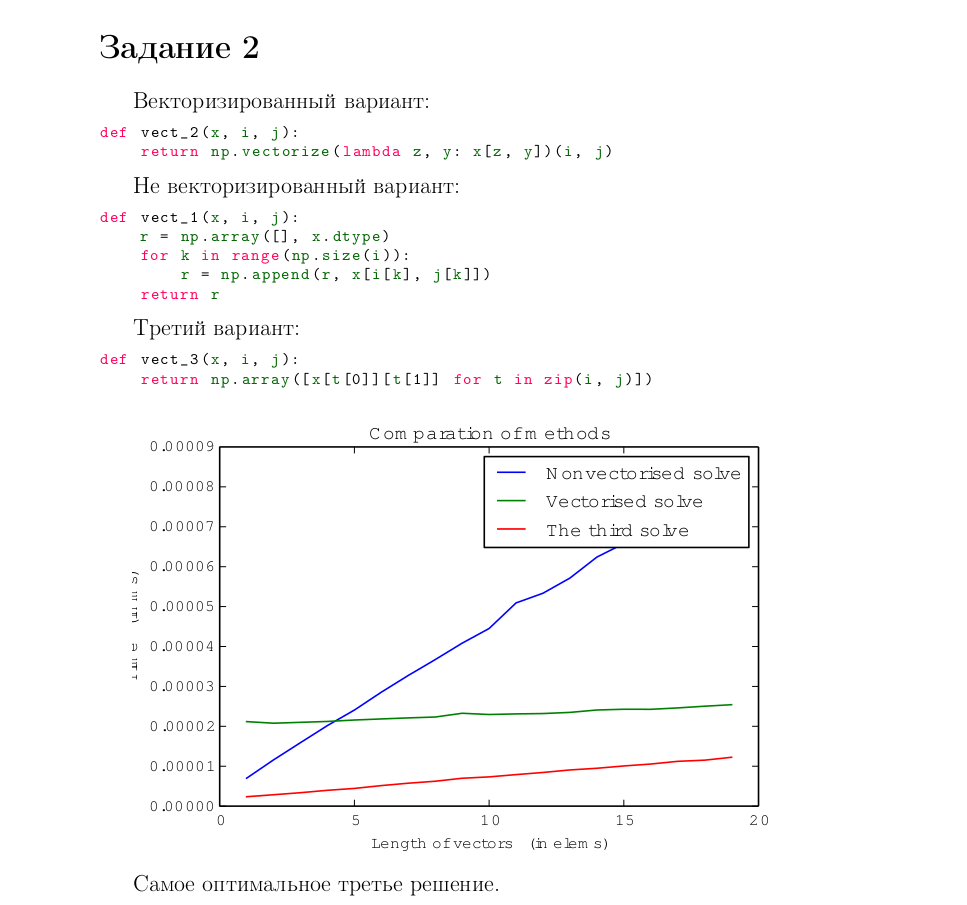
\includegraphics[height=6.5cm]{no_reason.png}}
\end{center}
Эксперименты не описаны, нет выводов.
\end{frame}

\begin{frame}{Описание экспериментов: как  надо делать}
\begin{center}
\fbox{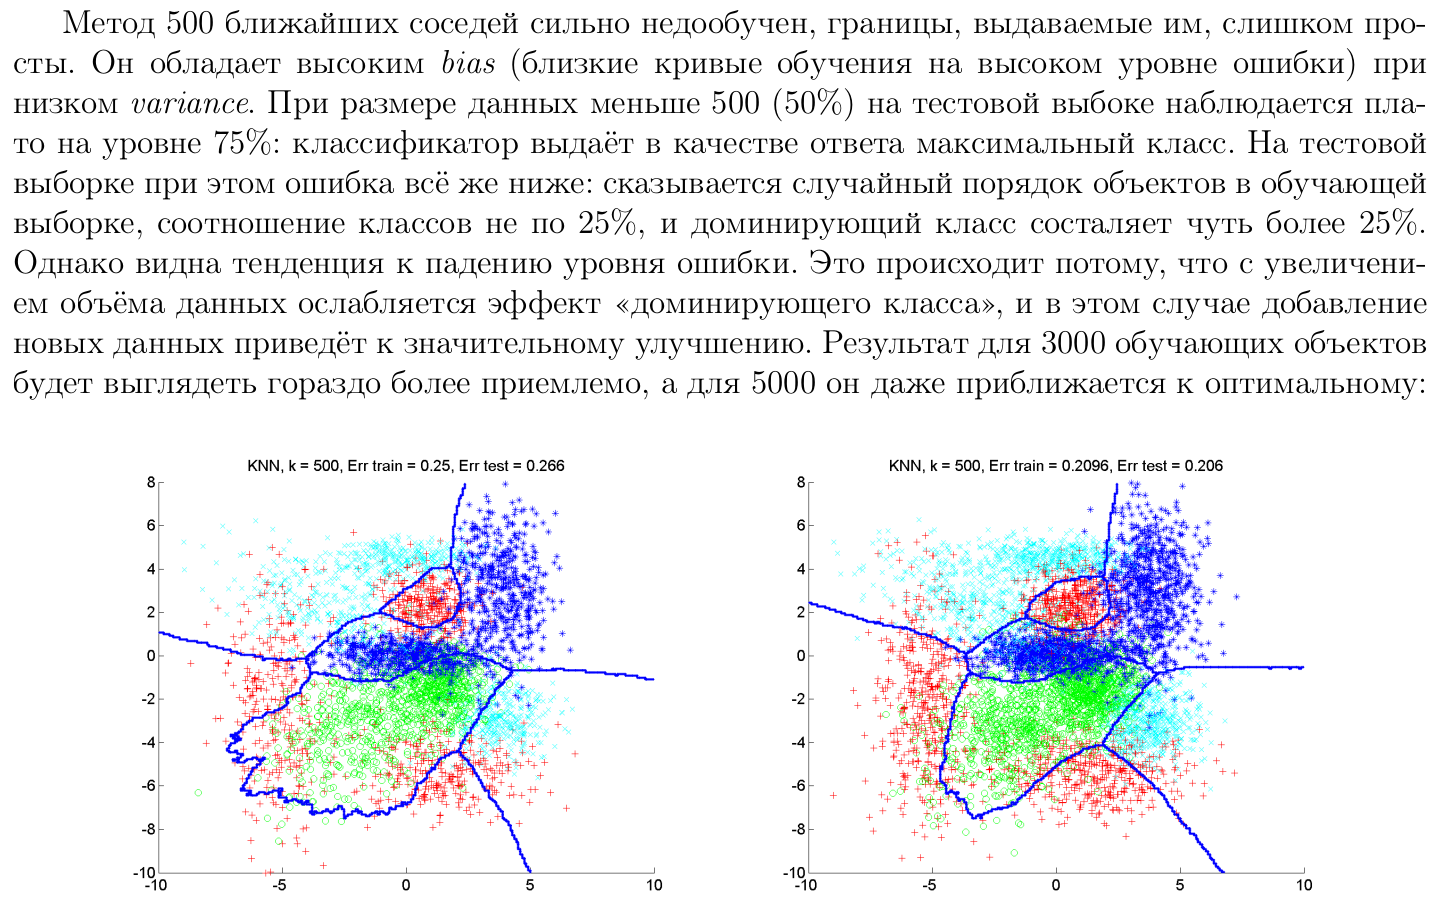
\includegraphics[height=6.5cm]{good_reason.png}}
\end{center}
Выводы проведены.
\end{frame}

\begin{frame}{Анализируйте результаты экспериментов}
\begin{table}[]
    \begin{tabular}{|c|c|c|c|}
        \hline
        размер данных & numpy & only python & смешанная \\ \hline
        10                                      & 1.2   & 50.21      & 2.1       \\ \hline
        100                                     & 2.52  & 40.1       & 10.2      \\ \hline
        1000                                    & 4.5   & 45.34      & 30.95     \\ \hline
    \end{tabular}
\end{table}

\hfill

\textcolor{red}{Что в этих результатах подозрительно?}

\hfill
\pause{
    \begin{itemize}
        \item Вычисления для размерности 100 и 1000 происходит быстрее чем для 10.
    \end{itemize}
}
\end{frame}

\begin{frame}{Используйте векторные шрифты}
\tabcolsep=10pt
\begin{tabular}{ll}
    Растровые шрифты: & Векторные шрифты: \\
    
\includegraphics[width=4.5cm]{bitmap_fonts.pdf} & 
\includegraphics[width=4.5cm]{vector_fonts.pdf}
\end{tabular}

\

Для генерации текстов с векторными шрифтами достаточно установить пакет \TeX\ \texttt{cm-super}.
\end{frame}

\end{subsection}

\begin{subsection}{Оформление графиков}

\begin{frame}{Оформление графиков. Некоторые советы}
    Графики должны быть с одной стороны понятными и информативными, а с другой стороны \textit{красивыми}.
    
	\begin{center}
		\fbox{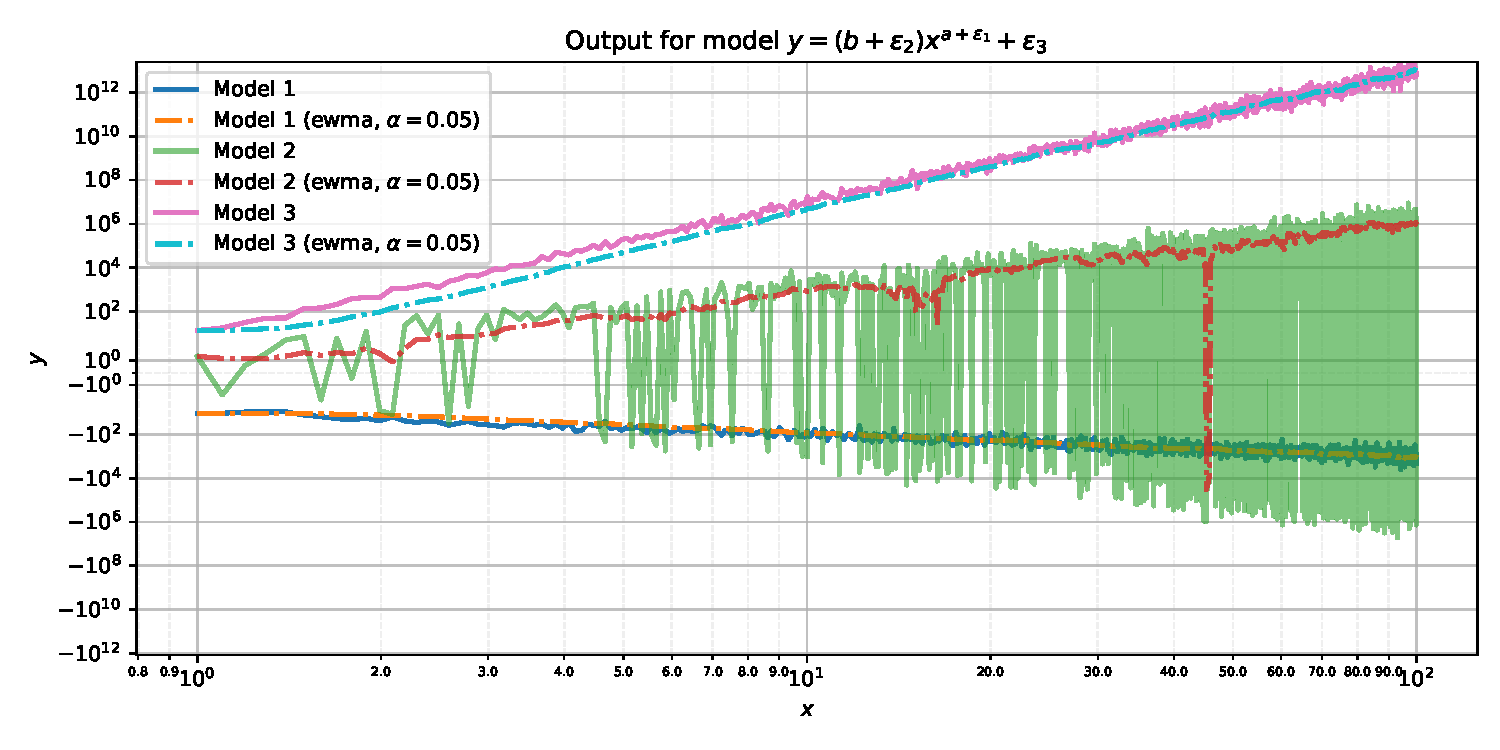
\includegraphics[height=5.5cm]{bad_plots/good_plot.pdf}}
	\end{center}
\end{frame}

\begin{frame}{Оформление графиков. Некоторые советы}
    \begin{itemize}
        \item Все графики должны быть отрисованы в векторном формате
    \end{itemize}
    
	\begin{center}
		\fbox{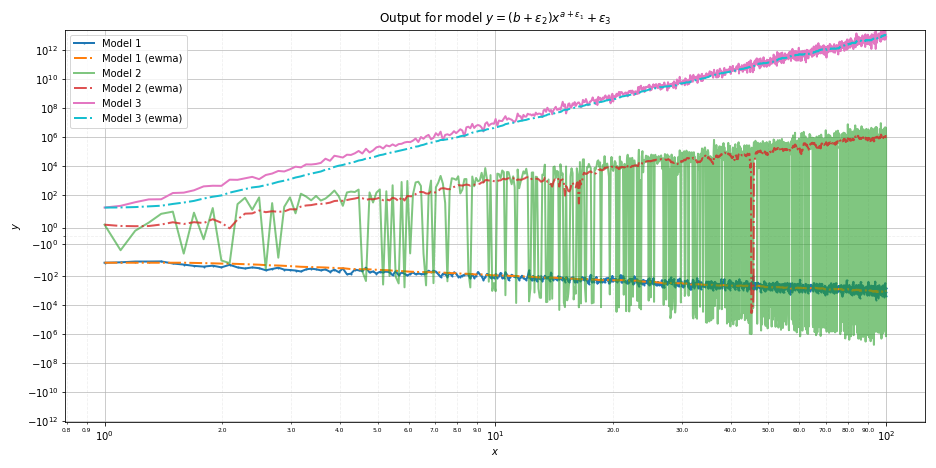
\includegraphics[height=5.5cm]{bad_plots/non_vector_plot.png}}
	\end{center}
\end{frame}

\begin{frame}{Оформление графиков. Некоторые советы}
    \begin{itemize}
        \item На всех графиках без исключения должна быть отрисована сетка
    \end{itemize}
    
	\begin{center}
		\fbox{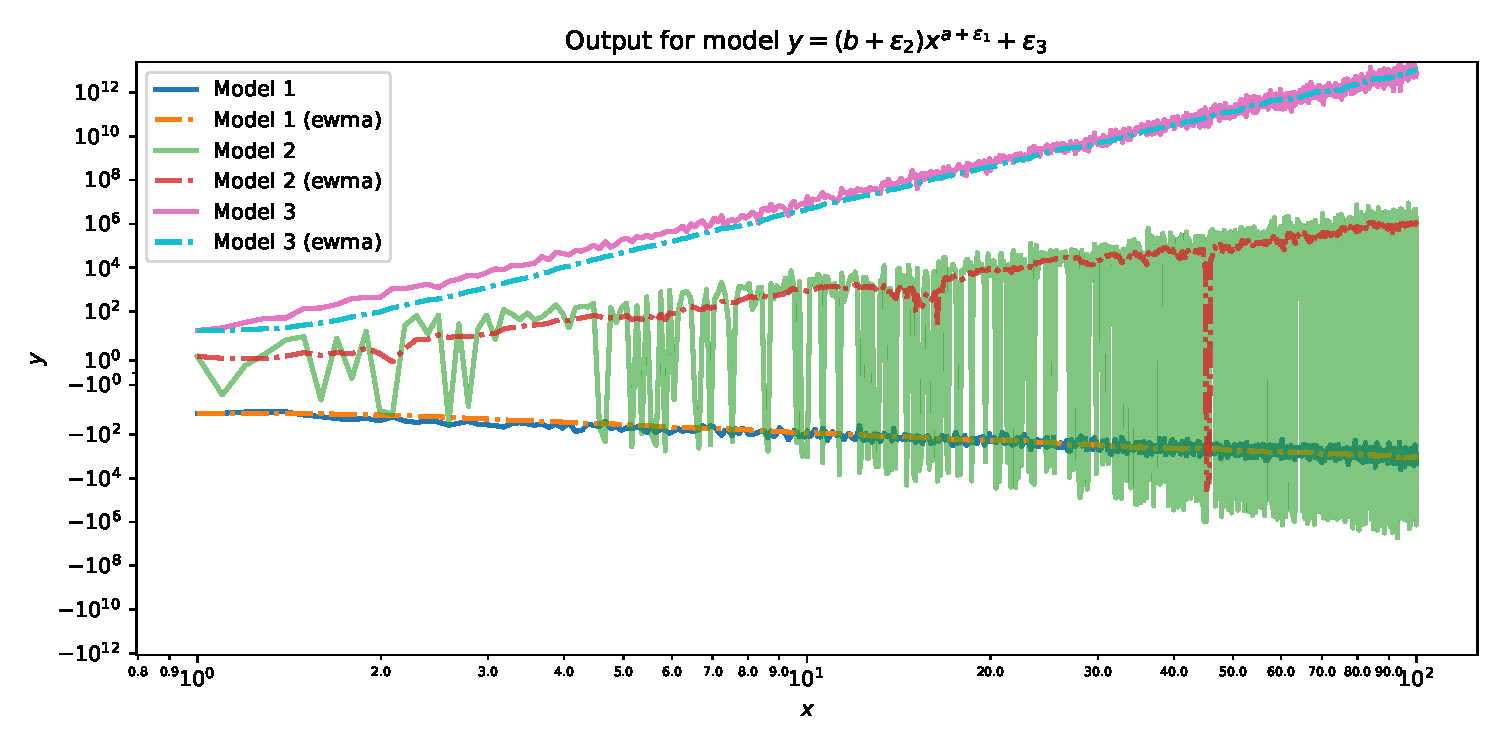
\includegraphics[height=5.5cm]{bad_plots/no_grid_plot.pdf}}
	\end{center}
\end{frame}

\begin{frame}{Оформление графиков. Некоторые советы}
    \begin{itemize}
        \item Все графики и группы графиков должны иметь заголовок
        \item При необходимости оси должны быть подписаны
        \item Если на графике отображено несколько сущностей, то необходима исчерпывающая легенда
    \end{itemize}
    
	\begin{center}
		\fbox{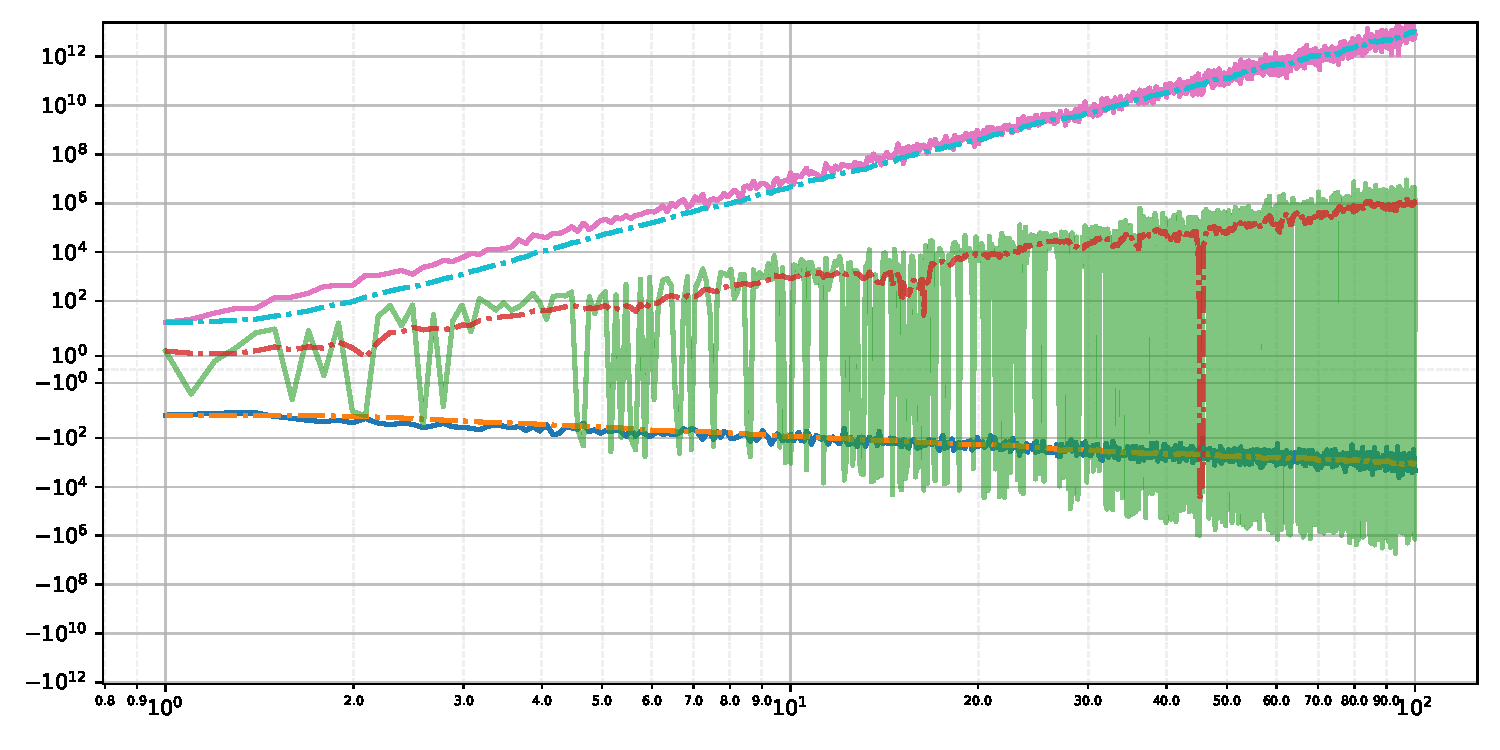
\includegraphics[height=5.5cm]{bad_plots/no_labels_plot.pdf}}
	\end{center}
\end{frame}

\begin{frame}{Оформление графиков. Некоторые советы}
    \begin{itemize}
        \item Все линии на графиках должны быть чётко видны
        \item Используйте \textit{красивую} цветовую палитру с хорошо различимыми цветами
    \end{itemize}
    
	\begin{center}
		\fbox{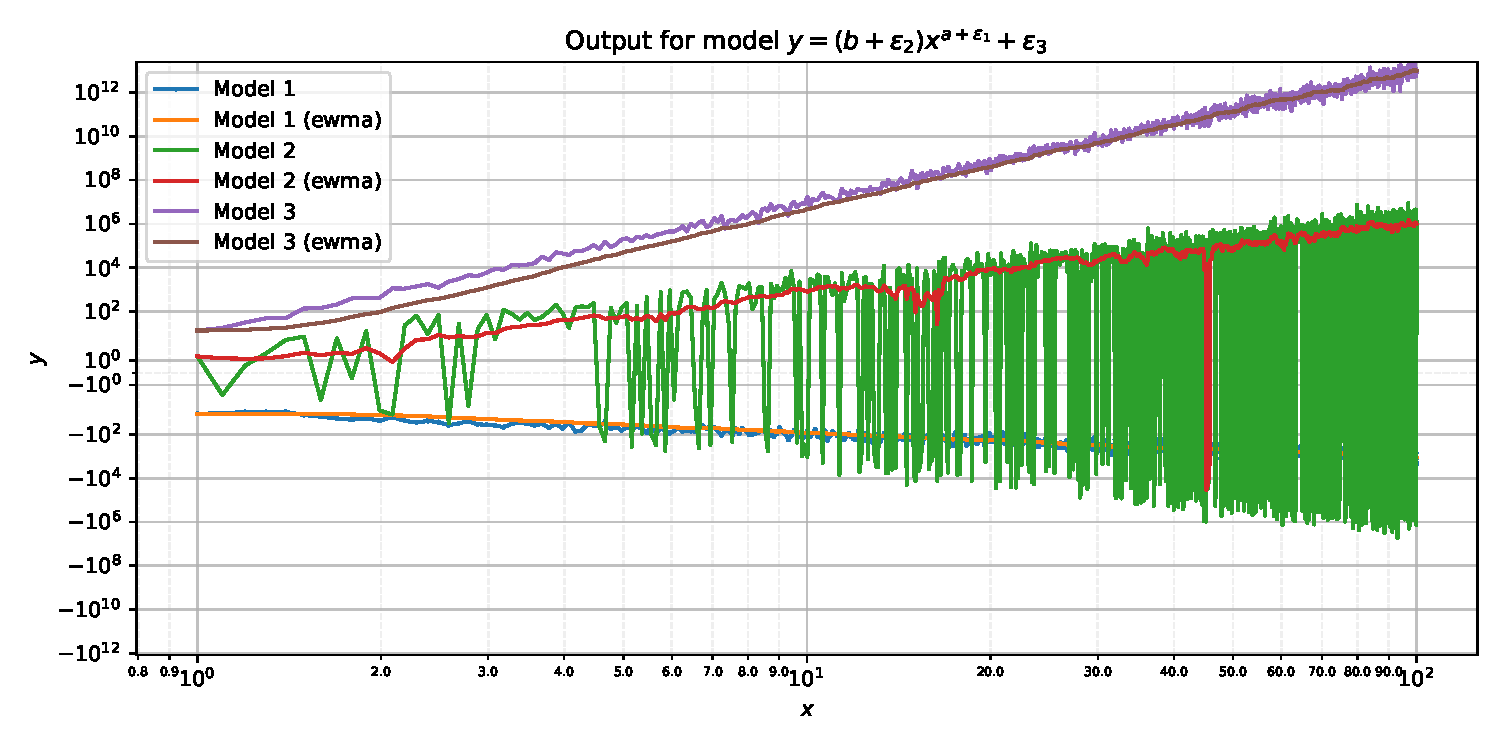
\includegraphics[height=5.5cm]{bad_plots/non_optimal_style_plot.pdf}}
	\end{center}
\end{frame}

\begin{frame}{Оформление графиков. Некоторые советы}
    \begin{itemize}
        \item Масштаб по каждой оси на графике должен быть выбран правильно
    \end{itemize}
    
	\begin{center}
		\fbox{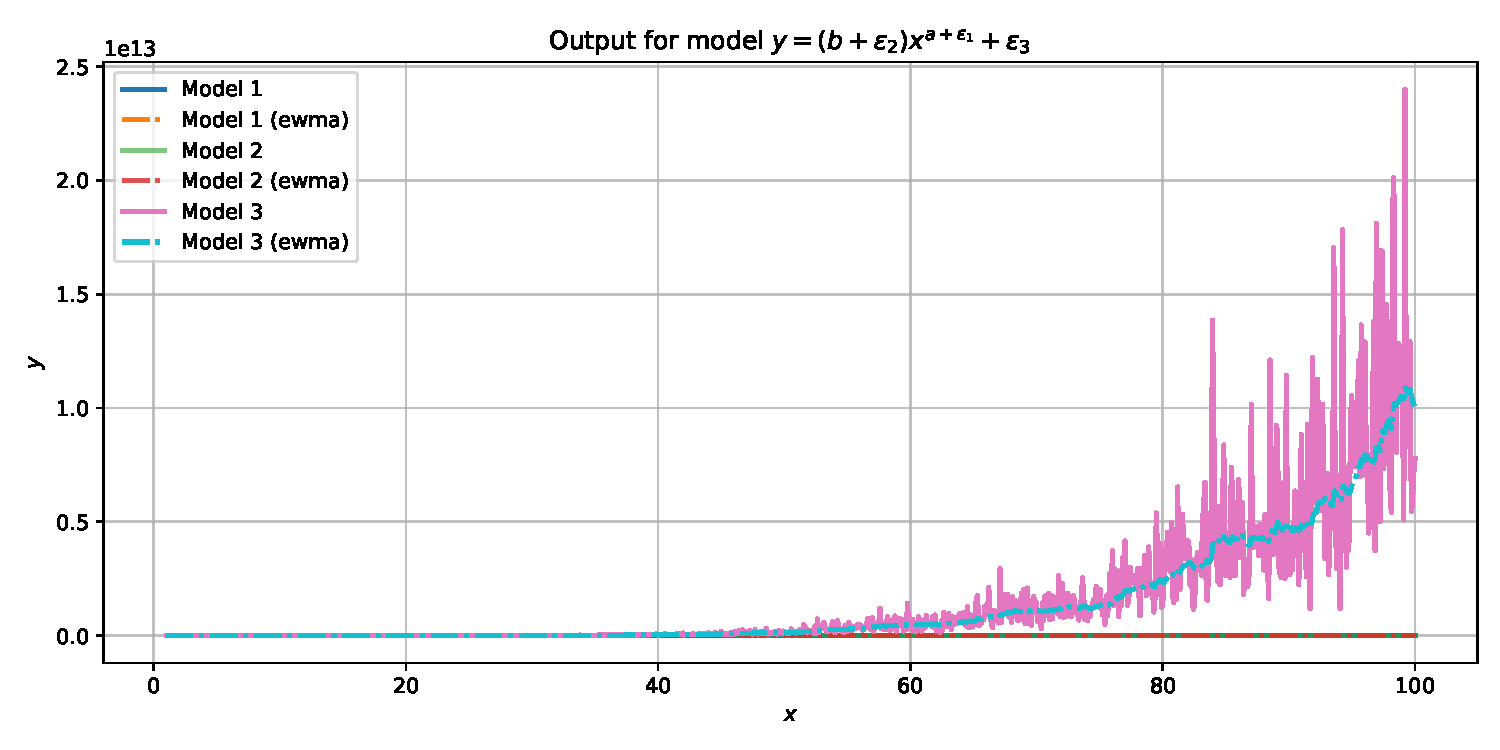
\includegraphics[height=5.5cm]{bad_plots/no_scaling_plot.pdf}}
	\end{center}
\end{frame}

\begin{frame}{Оформление графиков. Некоторые советы}
    \begin{itemize}
        \item Написания формул в заголовках, легенде и в подписях осей необходимо выполнять с помошью LaTeX
    \end{itemize}
    
	\begin{center}
		\fbox{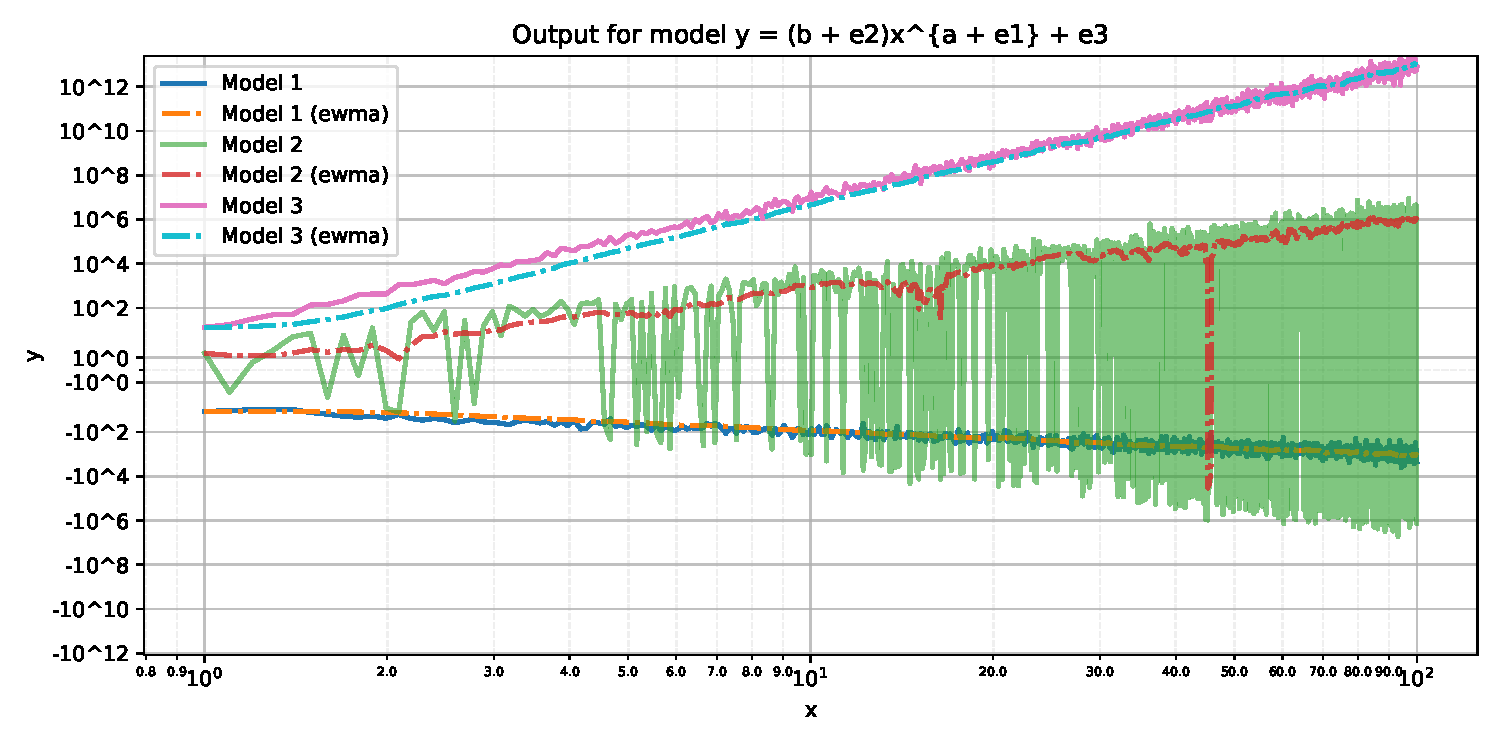
\includegraphics[height=5.5cm]{bad_plots/no_latex_plot.pdf}}
	\end{center}
\end{frame}

\begin{frame}{Оформление графиков. Некоторые советы}
    \begin{itemize}
        \item Графики должны быть не супер-микро и не супер-макро по размерам, так, чтобы можно было увидеть все, что нужно    
    \end{itemize}
    
	\begin{center}
		\fbox{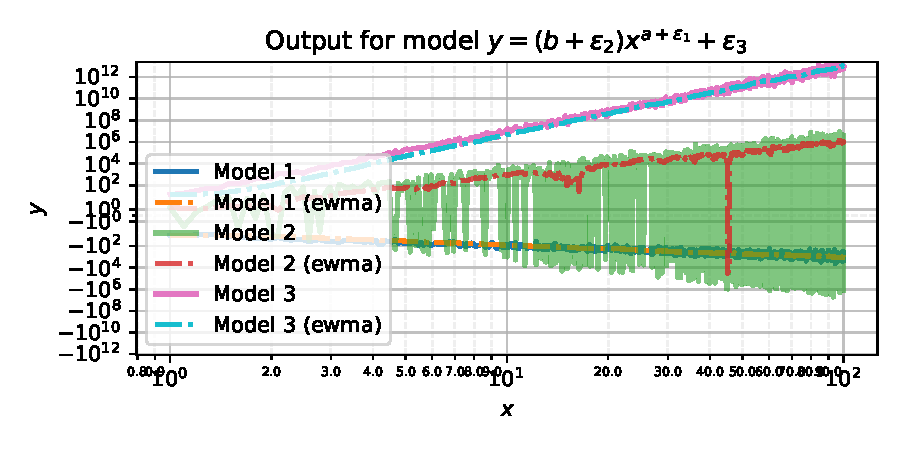
\includegraphics[height=3.5cm]{bad_plots/no_resize_plot.pdf}}
	\end{center}
\end{frame}

\begin{frame}{Оформление графиков. Примеры из жизни}
	\begin{center}
		\fbox{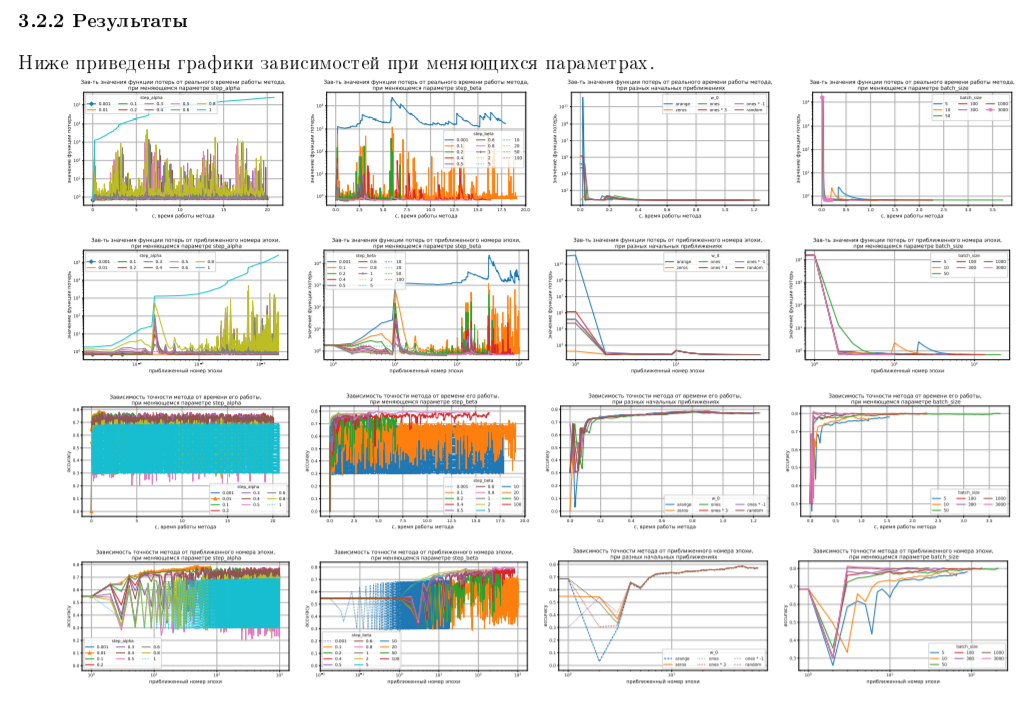
\includegraphics[height=6.5cm]{small_plots.png}}
	\end{center}
	Много подробных графиков, но все они нечитаемы!
\end{frame}

\begin{frame}{Оформление графиков. Примеры из жизни}
	\begin{center}
		\fbox{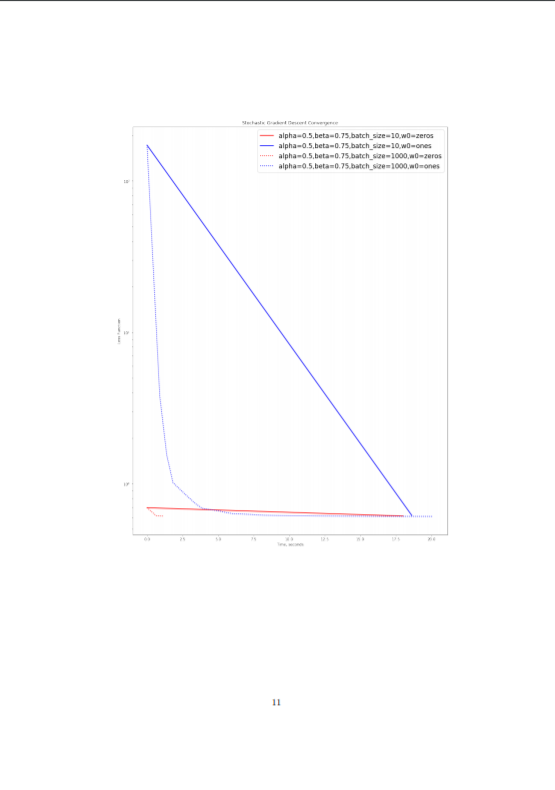
\includegraphics[height=6cm]{huge_plots.png}}
	\end{center}
	Тут -- наоборот, большой график, но понять что на нём происходит нельзя.
\end{frame}

\begin{frame}{Оформление графиков. Примеры из жизни}
	\begin{center}
		\fbox{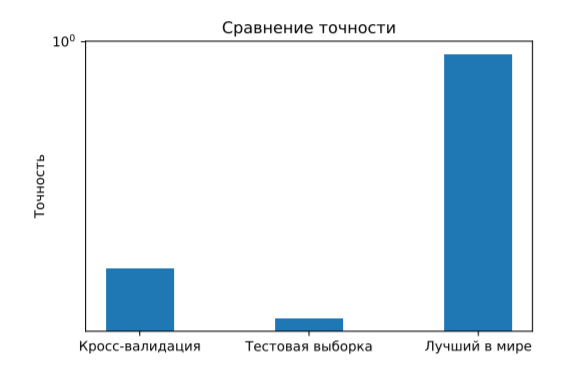
\includegraphics[height=6.5cm]{missing_ticks.png}}
	\end{center}
	Плохо подобраны отсчёты на вертикальной шкале.
\end{frame}

\begin{frame}{Оформление графиков. Примеры из жизни}
	\begin{center}
		\fbox{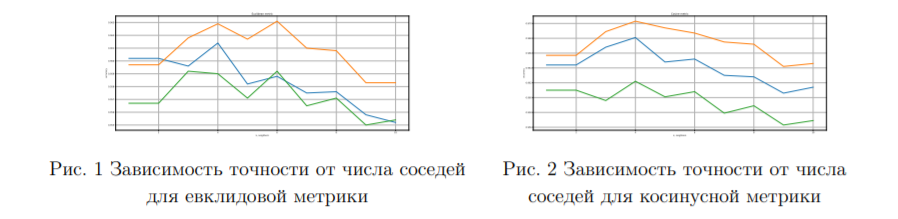
\includegraphics[height=2.5cm]{extra_small_ticks.png}}
	\end{center}
	Отсчёты не видно.
\end{frame}

\begin{frame}{Оформление графиков. Примеры из жизни}
\begin{center}
	\fbox{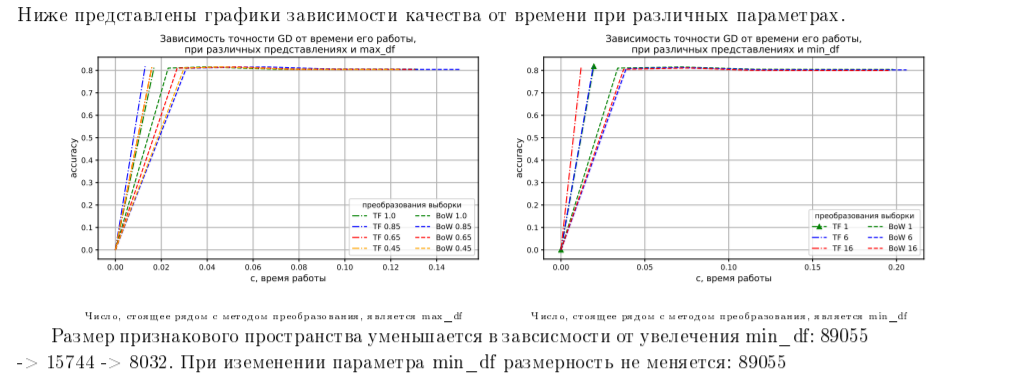
\includegraphics[height=4.0cm]{small_ticks.png}}
\end{center}
Подпись графика слишком мелкая.
\end{frame}

\begin{frame}{Оформление графиков. Примеры из жизни}
\begin{center}
    \tabcolsep=15pt
    \begin{tabular}{ll}
        Плохой график: & Хороший график: \\
        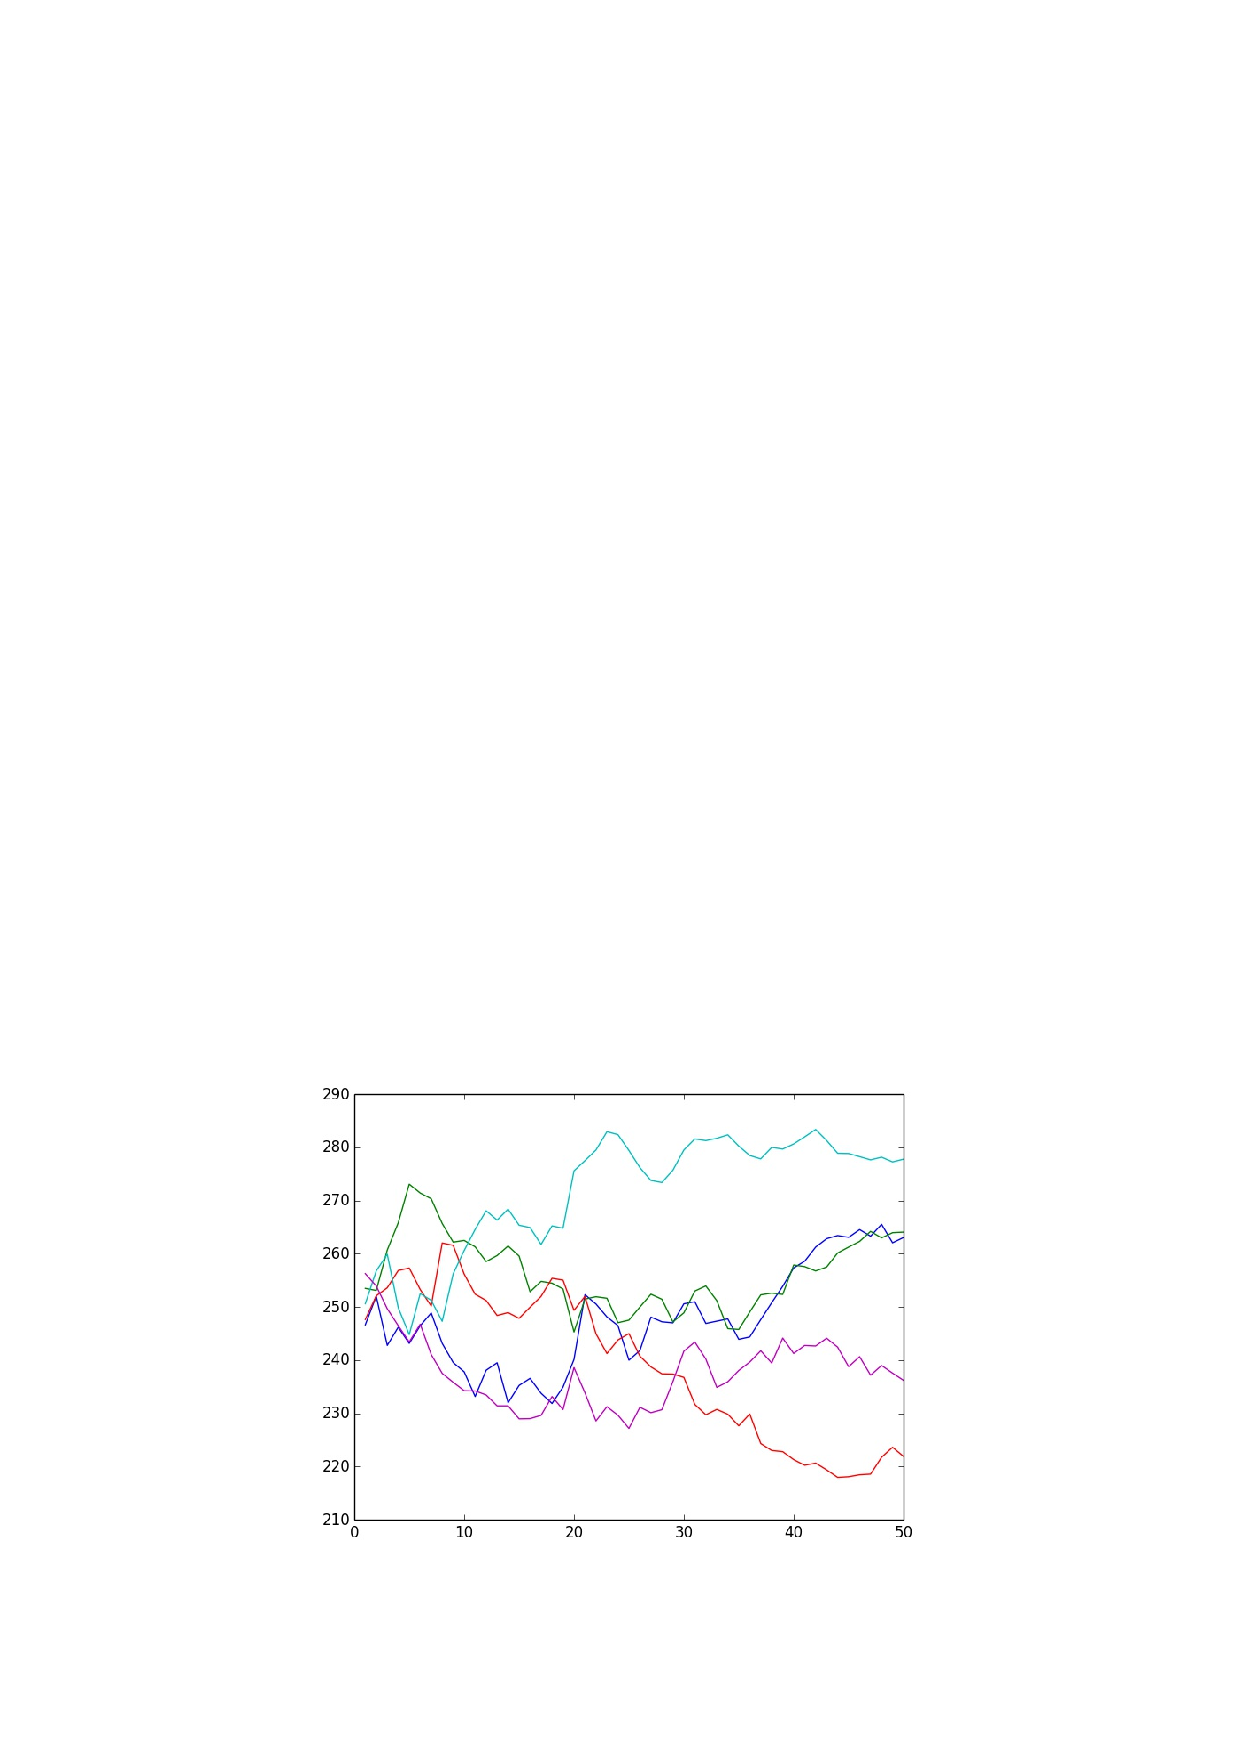
\includegraphics[height=3.5cm]{bag_picture.pdf} & 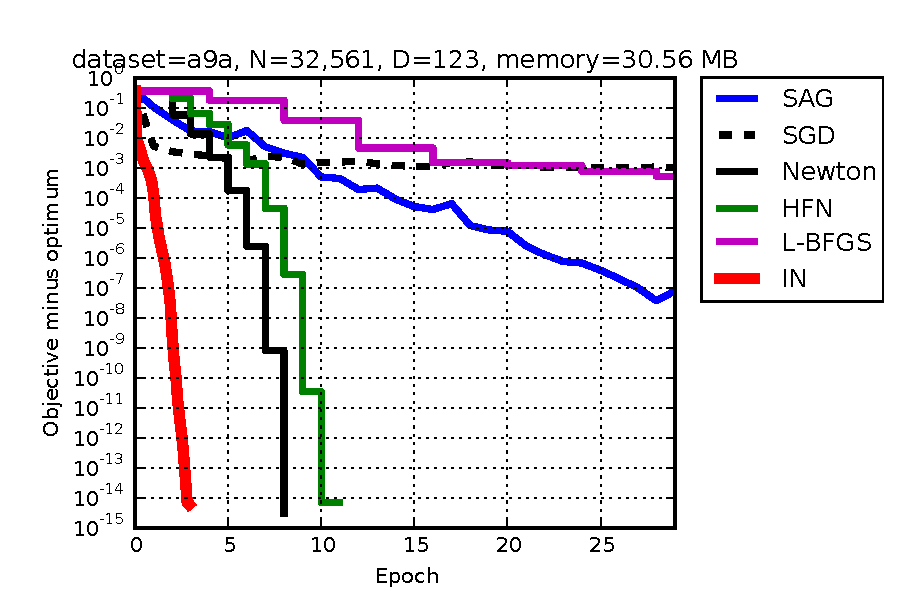
\includegraphics[height=3.5cm]{a9a_epoch.pdf}
    \end{tabular}
\end{center}

Элементы хорошего графика:
\begin{itemize}
    \item Все линии жирные;
    \item Есть легенда;
    \item По осям указаны значения, сами оси подписаны;
    \item По осям выбрана правильная шкала;
    \item Сохранён в векторном формате.
\end{itemize}

\end{frame}

\begin{frame}{Оформление графиков. Примеры из жизни}
	Хороший график:
	\begin{center}
		\fbox{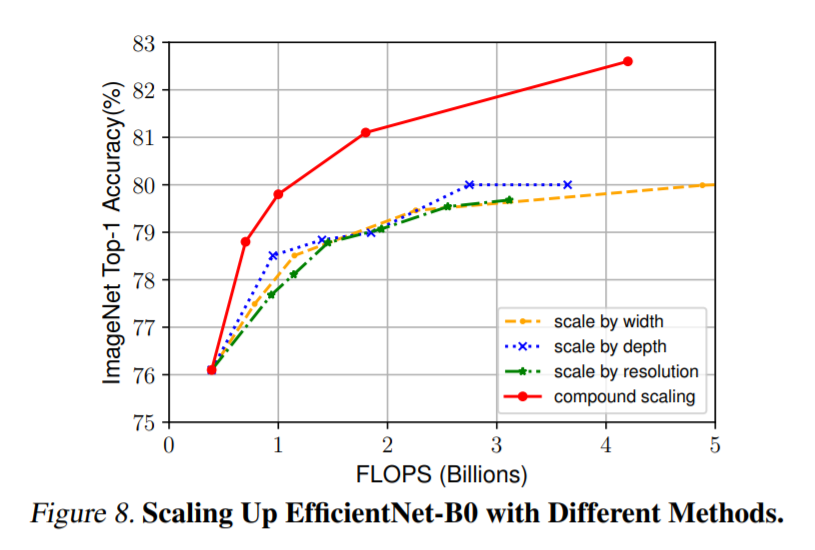
\includegraphics[height=5.0cm]{good_plot.png}}
	\end{center}
\end{frame}

\begin{frame}{Оформление графиков. Примеры из жизни}
	Хороший график:
	\begin{center}
		\fbox{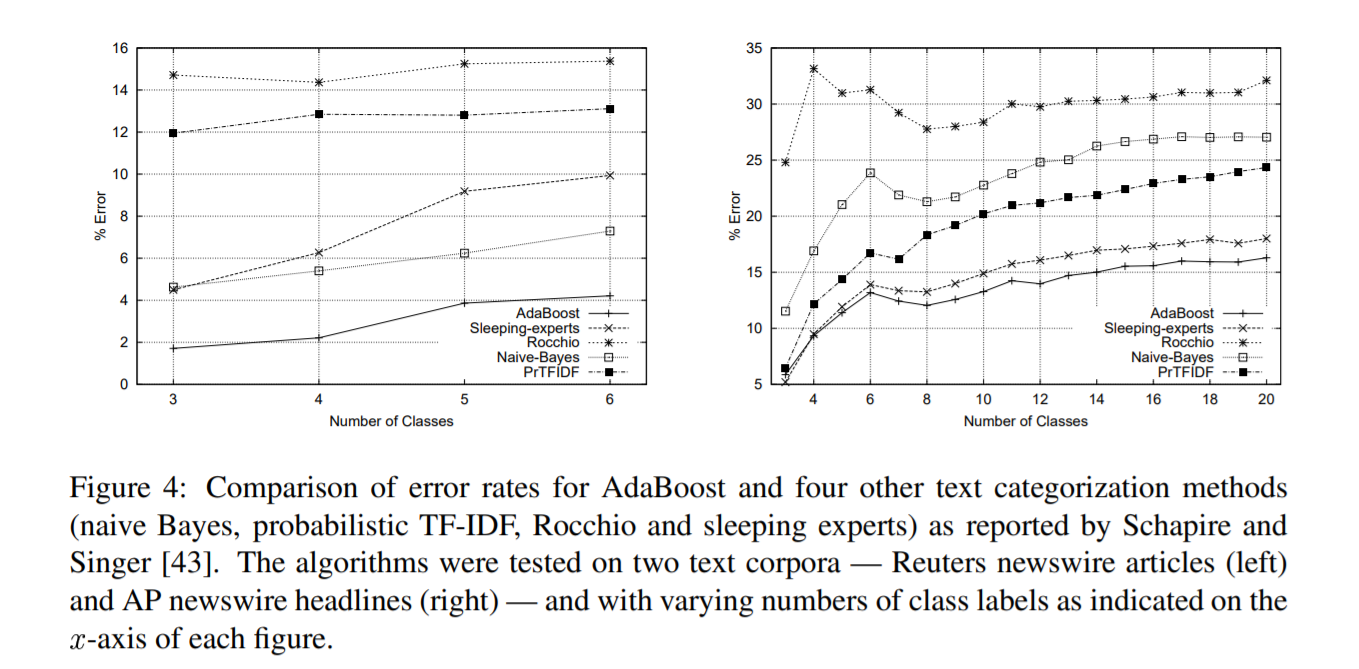
\includegraphics[height=5.0cm]{good_plot_black.png}}
	\end{center}
	Стоит задумываться о том, как будет выглядеть график, если он будет отображаться чёрно-белым.
\end{frame}

\begin{frame}{Думайте об оформлении результатов}
    \begin{center}
        {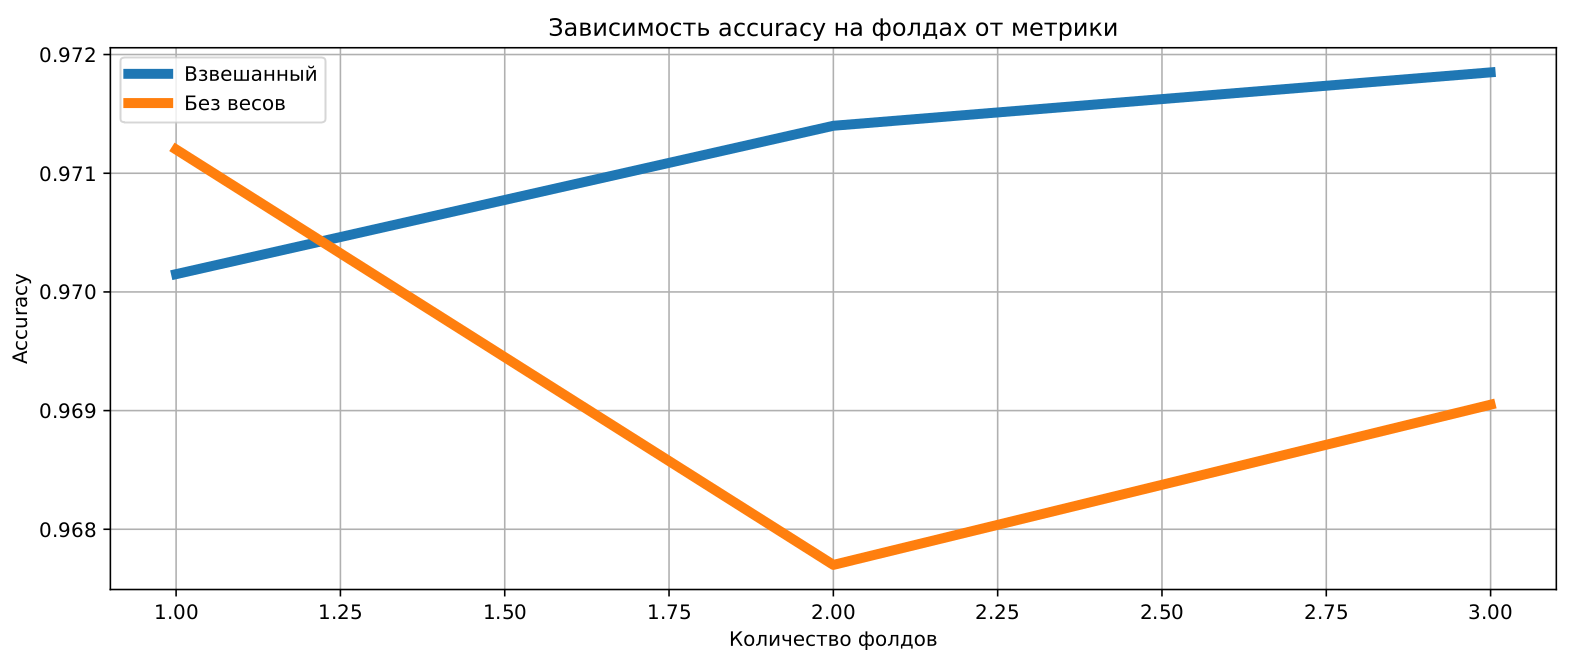
\includegraphics[height=4.8cm]{bad_graphic.png}}
    \end{center}
    
    \hfill
    
    \textcolor{red}{Что плохо на этой картинке?}
    \pause{
        Почти всё:
        \begin{itemize}
            \item Нет отношения порядка на оси x, опечатки, слишком подробная шкала.
        \end{itemize}
    }
    \end{frame}

\end{subsection}

\begin{subsection}{Огранизация страниц}

\begin{frame}{Примеры плохо организованных страниц}
	\begin{center}
		\fbox{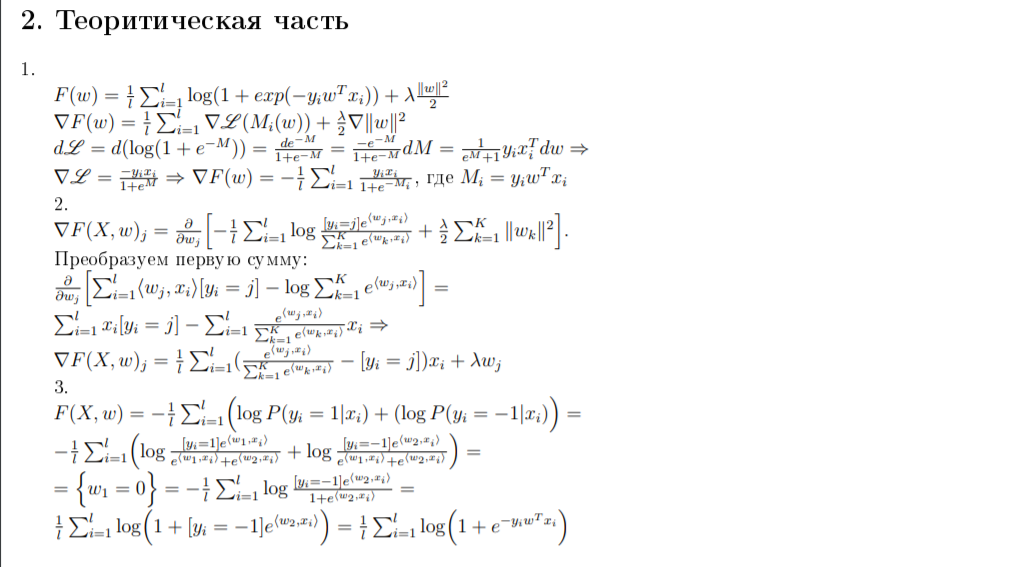
\includegraphics[height=5.0cm]{bad_formating.png}}
	\end{center}
	Формулы <<съехали>> и стали плохо читаться.
\end{frame}

\begin{frame}{Примеры плохо организованных страниц}
	\begin{center}
		\fbox{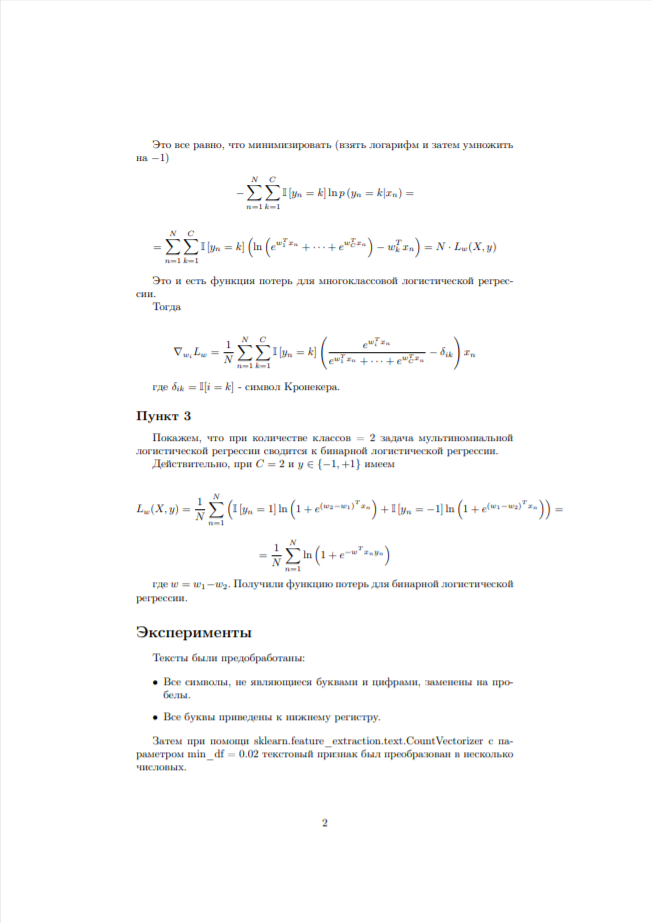
\includegraphics[height=6.5cm]{huge_borders.png}}
	\end{center}
	Слишком большие поля.
\end{frame}

\begin{frame}{Примеры плохо организованных страниц}
\begin{center}
\fbox{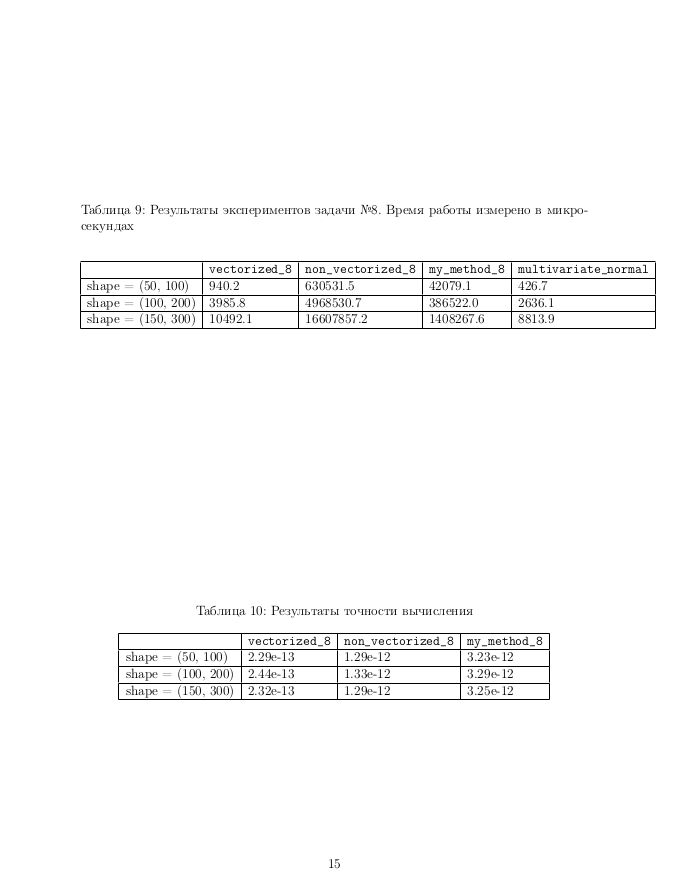
\includegraphics[height=6.5cm]{bad_page.png}}
\end{center}
Есть большие пустые пространства на странице.
\end{frame}

\begin{frame}{Примеры плохо организованных страниц}
\begin{center}
    \fbox{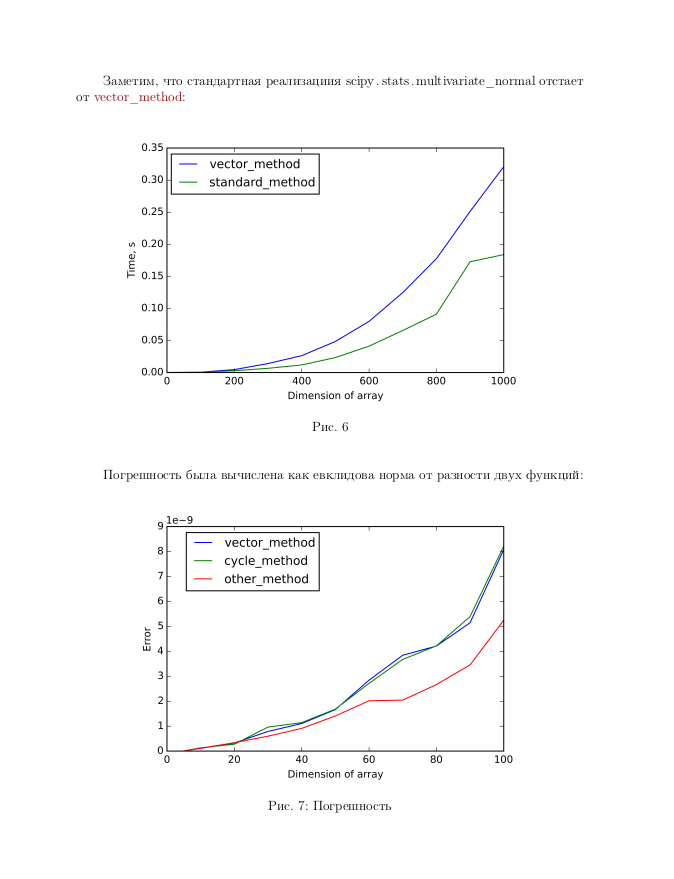
\includegraphics[height=6.5cm]{bad_page2.png}}
\end{center}
Графики занимают слишком много места.
\end{frame}

\begin{frame}{Примеры плохо организованных страниц}
\begin{center}
\fbox{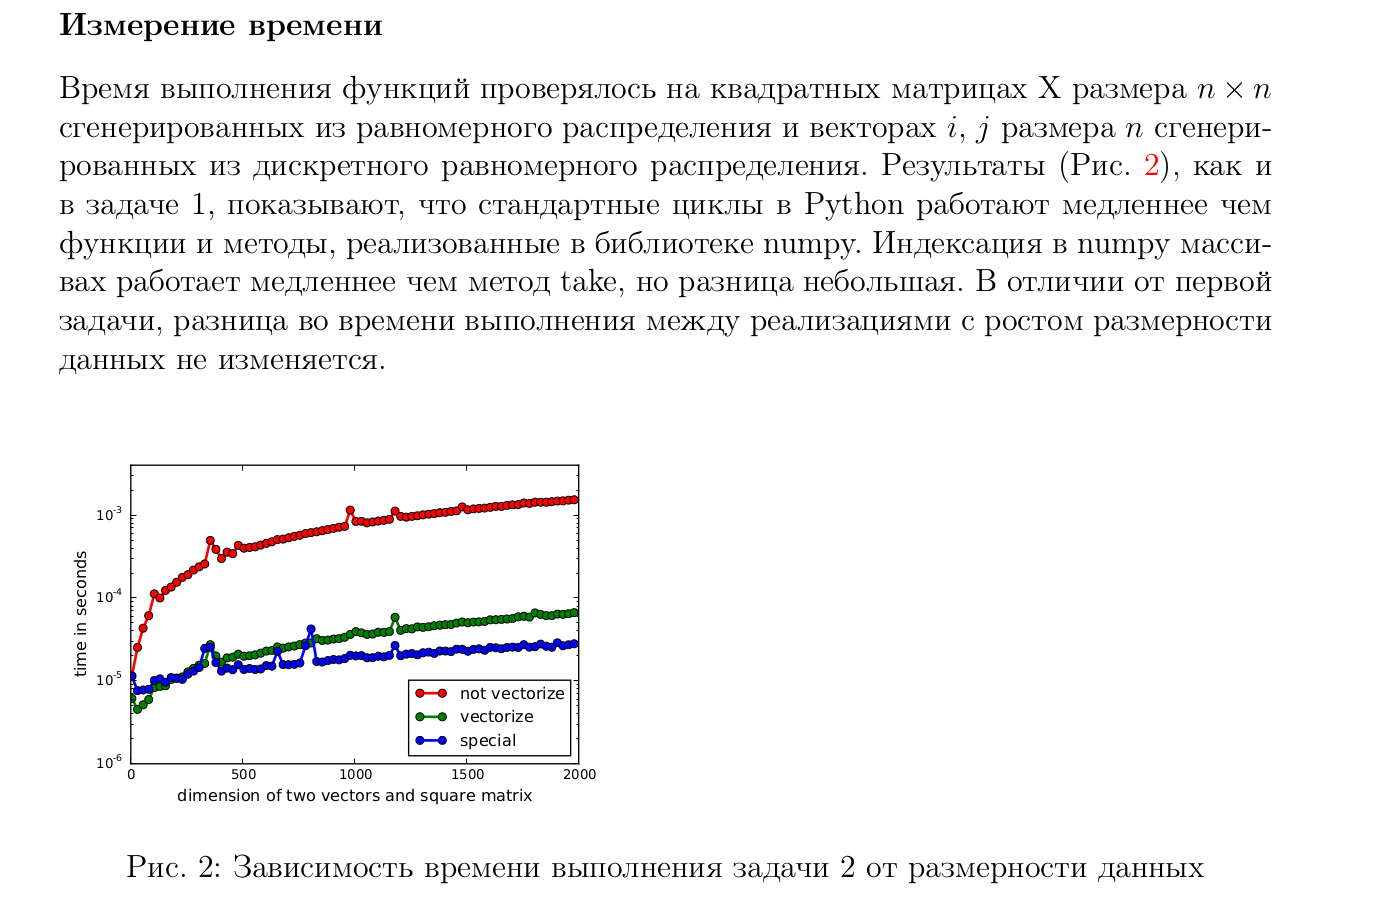
\includegraphics[height=5cm]{bad_page5.png}}
\end{center}

Есть большие пустые пространства на странице.
\end{frame}

\begin{frame}{Примеры плохо организованных страниц}
\begin{center}
\fbox{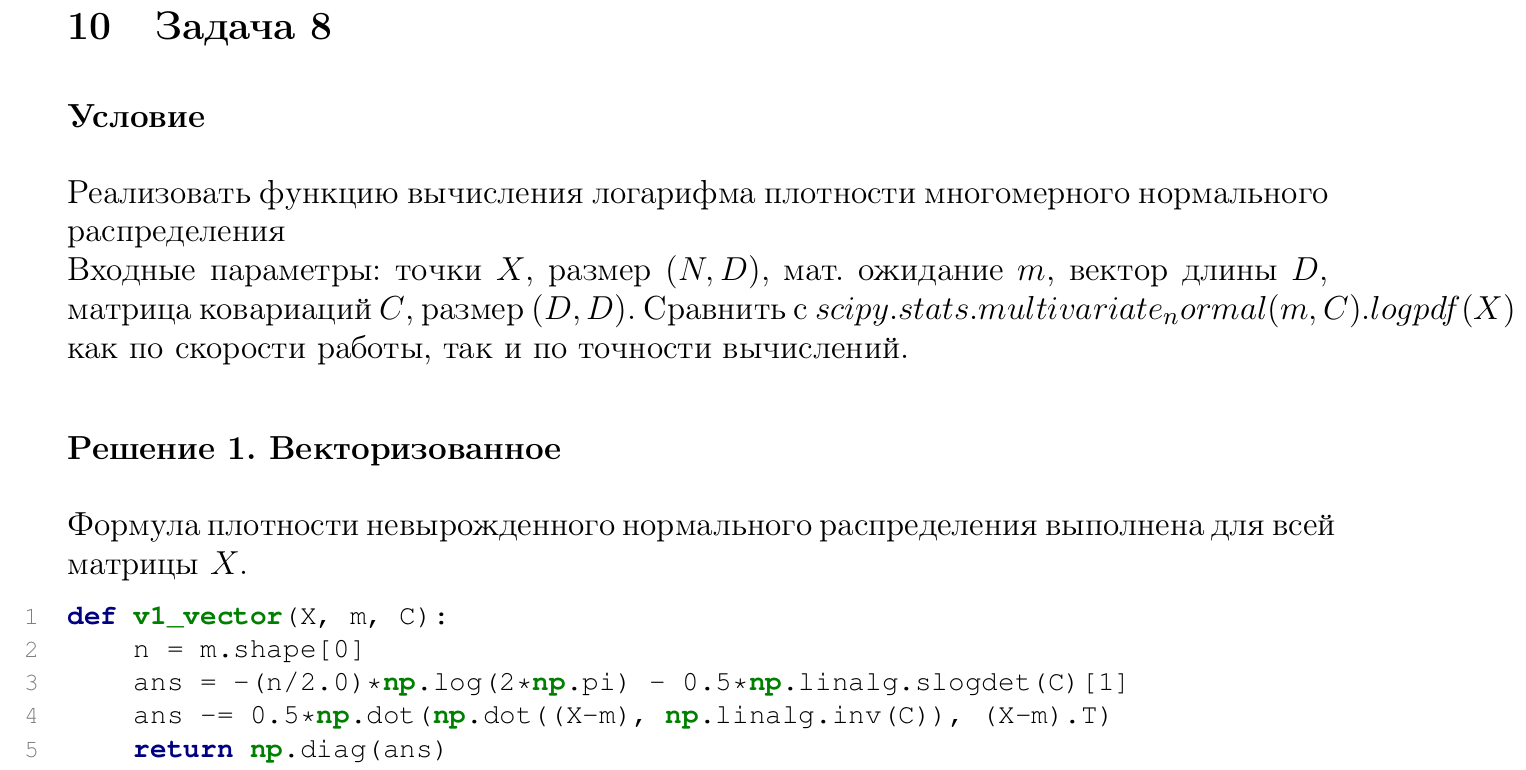
\includegraphics[height=5cm]{bad_page3.png}}
\end{center}
\end{frame}

\begin{frame}{Пример хорошо организованных страниц}
	\begin{center}
		\begin{tabular}{ll}
			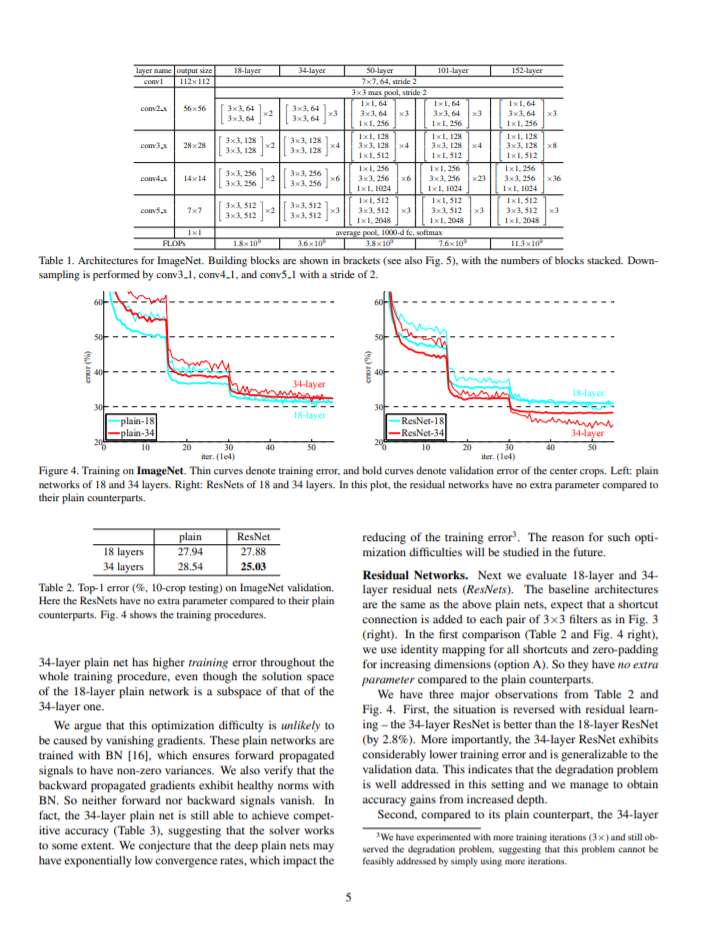
\includegraphics[height=7.5cm]{good_formatting.png} & 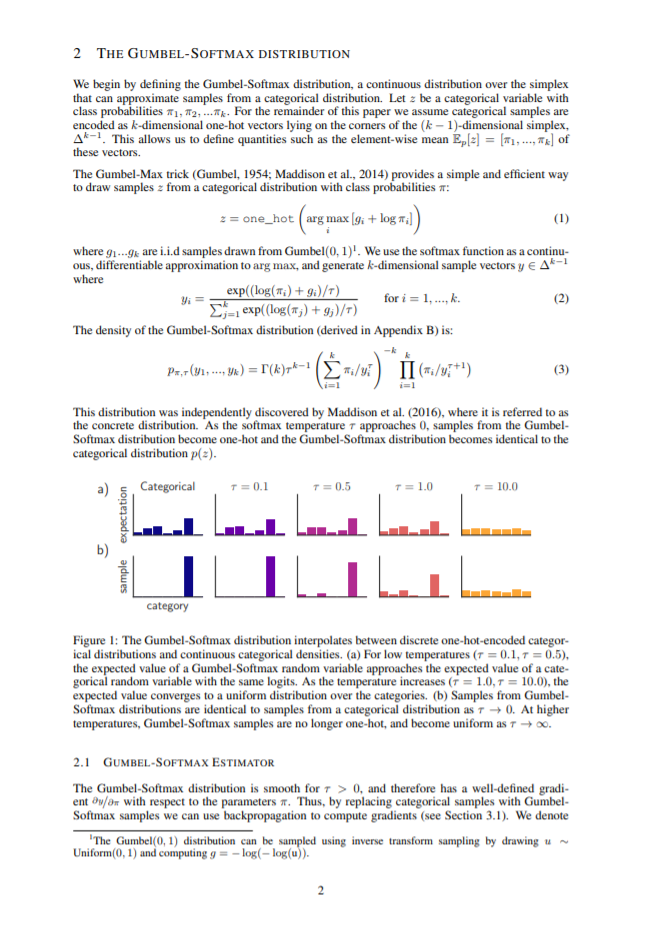
\includegraphics[height=7.5cm]{good_formatting_2.png}
		\end{tabular}
	\end{center}
\end{frame}

\end{subsection}


\begin{frame}{Все числа указываются с необходимым числом знаков}
\begin{center}
    {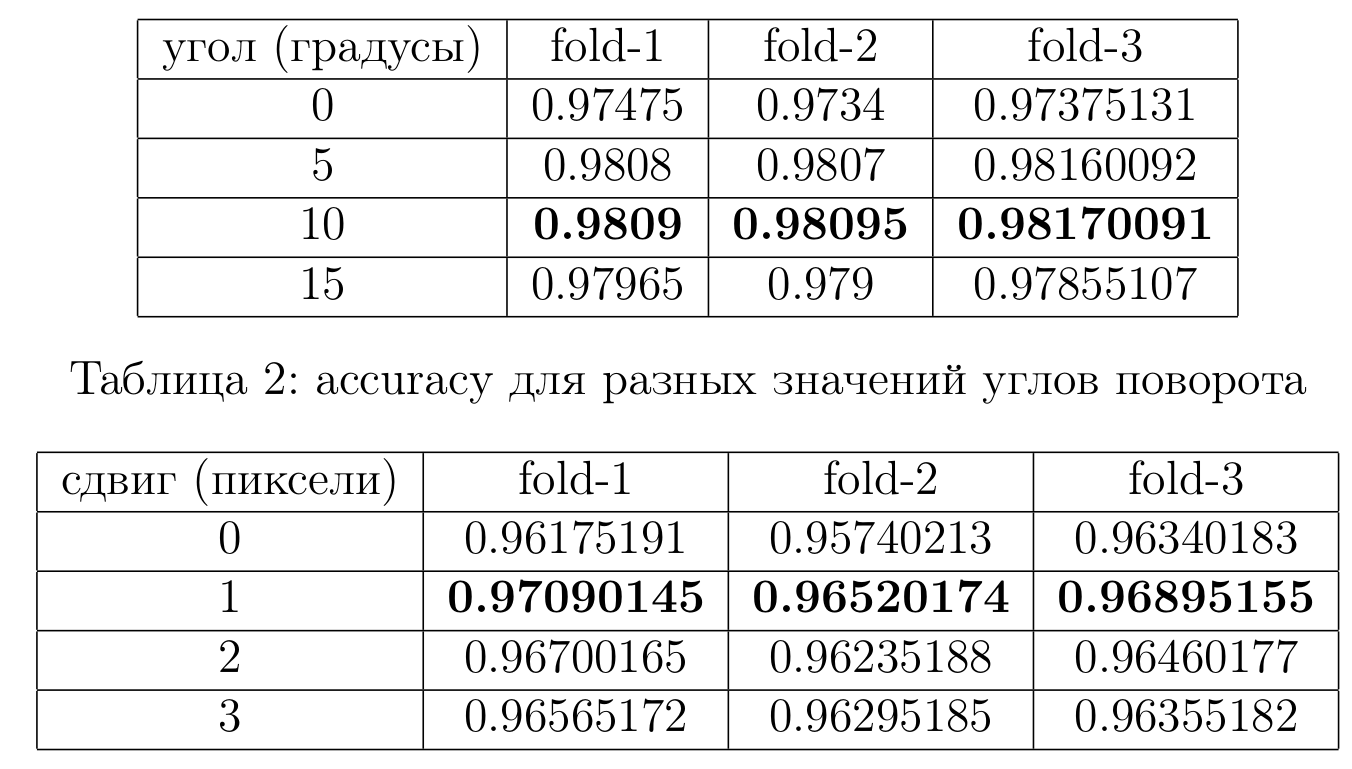
\includegraphics[height=6.5cm]{bad_numbers.png}}
\end{center}

Число указывается с точностью до 2 или 3 знака после запятой.
\end{frame}


\begin{frame}{Избегайте длинных предложений}
Далее в опытах, для настройки нашего метода, подбора оптимальных параметров, нам придётся использовать кросс-валидацию. Но эта операция занимает очень много времени, поэтому так как все стратегии, перечисленные выше, являются точными, то есть одинаково классифицируют один объект, имея одинаковую обучающую выборку, нам нужно измерить время их работы, и определить лучшую стратегию. Результат опыта на ниже приведнном рисунке.

\end{frame}

\begin{frame}{Чего ещё следует избегать?}
\begin{itemize}
    \item Ненаучной лексики (<<результаты модели получились фиговые>>) 
    \item Орфографических ошибок (установите проверку в среде)
    \item Грамматических, синтаксических и других ошибок
    \item Повествование от первого лица единственного числа
    \item Обращений к читателю (<<вашему вниманию представлены результаты экспериментов>>>)
    \item Смешения стиля использования буквы <<ё>> (либо везде используете <<ё>>, либо везде <<е>>)
\end{itemize}
\end{frame}

\begin{frame}{Итог: элементы хорошего отчёта по заданию}
\begin{itemize}
    \item Отчёт подготовлен в системе \TeX;
    \item Объём отчёта: 5--20 страниц;
    \item Текст отчёта не повторяет полной формулировки задания;
    \item Структура отчёта соответствует пунктам задания;
    \item Используются векторные шрифты;
    \item Графики оформлены надлежащим образом;
    \item Шкала для графиков выбрана правильно;
    \item На разных графиках результаты для одинаковых методов отображаются одним и тем же цветом;
\end{itemize}
\end{frame}

\begin{frame}{Итог: элементы хорошего отчёта по заданию}
\begin{itemize}
\item Между расположением графиков и местами их упоминания в тексте относительно небольшое расстояние (на той же или на соседней странице);
\item На страницах не должно быть много пустого места;
\item В большинстве случаев графики/таблицы/псевдокоды алгоритмов не должны занимать большей части одной страницы отчёта;
\item Все числа в тексте/таблицах указаны с необходимым числом значащих цифр;
\item В большинстве случае в отчёте не должно быть никакого кода;
\item Для всех экспериментов описан выбранный дизайн экспериментов, а также сделаны выводы из полученных результатов;
\end{itemize}
\end{frame}

\section{Система разметки \TeX}
\subsection*{}

\begin{frame}{Система \TeX}
\TeX~--- система компьютерной вёрстки, построенная по принципу компиляции документа, записанного с помощью специального языка разметки.

\

Изобретена Д. Кнутом в конце 70х годов.

\

Является де-факто стандартом для написания научных статей.

\

Язык разметки \TeX\ используется для набора формул во многих системах: в вики-разметке, в matplotlib, Microsoft Office и др.

\

\LaTeX --- надстройка поверх \TeX.
\end{frame}

\begin{frame}{Дистрибутивы и редакторы \TeX}
Дистрибутивы:
\begin{itemize}
    \item Windows: MiKTeX, TeX Live
    \item Linux: TeX Live
    \item Mac OS: MacTeX, TeX Live
\end{itemize}

\hfill

Редакторы: WinEdt, TeXnicCenter, Kile, TeXmaker, TeXstudio \ldots

\end{frame}

\begin{frame}{Дистрибутивы и редакторы \TeX}
    Рекомендуемые редакторы:
    \begin{itemize}
        \item VSCode + Latex Workshow. \href{https://youtu.be/DL70VzEqY5Y}{Инструкция по установке}
        \item TeXstudio
        \item Overleaf -- облачный редактор. \href{https://ru.overleaf.com/learn/latex/LaTeX_video_tutorial_for_beginners_(video_1)}{Туториал}
    \end{itemize}
\end{frame}

\begin{frame}{Режимы компиляции}

\begin{itemize}
    \item \texttt{tex -> dvi -> ps -> pdf}
    
    \item \texttt{tex -> dvi -> pdf}
    
    \item \texttt{tex -> pdf}
\end{itemize}
\end{frame}

\begin{frame}[fragile]{Структура файла .tex}
\begin{lcode}
\documentclass{article} % класс документа
%Преамбула документа
\usepackage[T2A]{fontenc} % задаём кодировку шрифтов
\usepackage[utf8x]{inputenc} % задаём кодировку файла
% задаём правила переносов для русского языка
\usepackage[english,russian]{babel}

% Текст документа
\begin{document}
Некоторый текст в первом абзаце.
Несколько      пробелов подряд считаются как один.

Конец абзаца задаётся задаётся пустой строкой.
\end{document}
\end{lcode}
\end{frame}

\begin{frame}[fragile]{Разделы и подразделы}
\begin{lcode}
\section{Раздел 1}
\subsection{Подраздел}
\subsubsection{Подподраздел}

\section{Раздел 2}
\end{lcode}
\end{frame}

\begin{frame}[fragile]{Окружения списков}
    \begin{lcode}
    \begin{itemize}
        \item Пункт
        \item Ещё один пункт
    \end{itemize}
    
    \begin{enumerate}
        \item Пункт 1
        \item Пункт 2
    \end{enumerate}
    \end{lcode}

    \begin{figure}[h!]
        \begin{minipage}[b]{0.45\textwidth}
            \begin{itemize}
                \item Пункт
                \item Ещё один пункт
            \end{itemize}
        \end{minipage}
        \begin{minipage}[b]{0.45\textwidth}
            \begin{enumerate}
                \item Пункт 1
                \item Пункт 2
            \end{enumerate}
        \end{minipage}
    \end{figure}

\end{frame}

\begin{frame}[fragile]{Формулы}

\begin{lcode}
Формула в тексте: $\sin^2x + \cos^2x = 1$.
\end{lcode}

Формула в тексте: $\sin^2x + \cos^2x = 1$.

\begin{lcode}
Выносная формула:
$$
A_{ij} = b_i^2 + c_j^3\quad \forall i,j=1,\dots,n.
$$
\end{lcode}

Выносная формула:
$$
A_{ij} = b_i^2 + c_j^3\quad \forall i,j=1,\dots,n.
$$

\end{frame}

\begin{frame}[fragile]{Формулы}

\begin{lcode}
Выравнивание по левому краю: \[ x^n + y^n = z^n \]
\end{lcode}

Выравнивание по левому краю: \[ x^n + y^n = z^n \]

\begin{lcode}
    \begin{equation}
        \sin^2x + \cos^2x = 1 \label{eq:trig_eq}
    \end{equation}
    Ссылка по метке: \ref{eq:trig_eq}
\end{lcode}

\begin{equation}
    \sin^2x + \cos^2x = 1 \label{eq:trig_eq}
\end{equation}
Ссылка по метке: \ref{eq:trig_eq}

\end{frame}

\begin{frame}[fragile]{Формулы}
\begin{lcode}
Выравнивание формул:
\begin{align}
\notag p(y|x) = \frac{p(x|y)p(y)}{p(x)} &= \\
\label{eq:bayes}&= \frac{1}{Z}p(x|y)p(y)
\end{align}
\end{lcode}

Выравнивание формул:
\begin{align}
\notag p(y|x) = \frac{p(x|y)p(y)}{p(x)} &= \\
\label{eq:bayes}&= \frac{1}{Z}p(x|y)p(y)
\end{align}

\end{frame}

\begin{frame}[fragile]{Ссылки}
\begin{lcode}
\begin{equation}
\label{eq::1}
E = mc^2.
\end{equation}

Ссылка на формулу~\eqref{eq::1}
\end{lcode}
\begin{equation}
\label{eq::1}
E = mc^2.
\end{equation}

Ссылка на формулу~\eqref{eq::1}

\begin{lcode}
\section{Ссылки}\label{sec:1}
Ссылка на раздел~\ref{sec:1} в документе.
\end{lcode}

\end{frame}

\begin{frame}[fragile]{Картинки}
\begin{lcode}
Картинка в тексте:
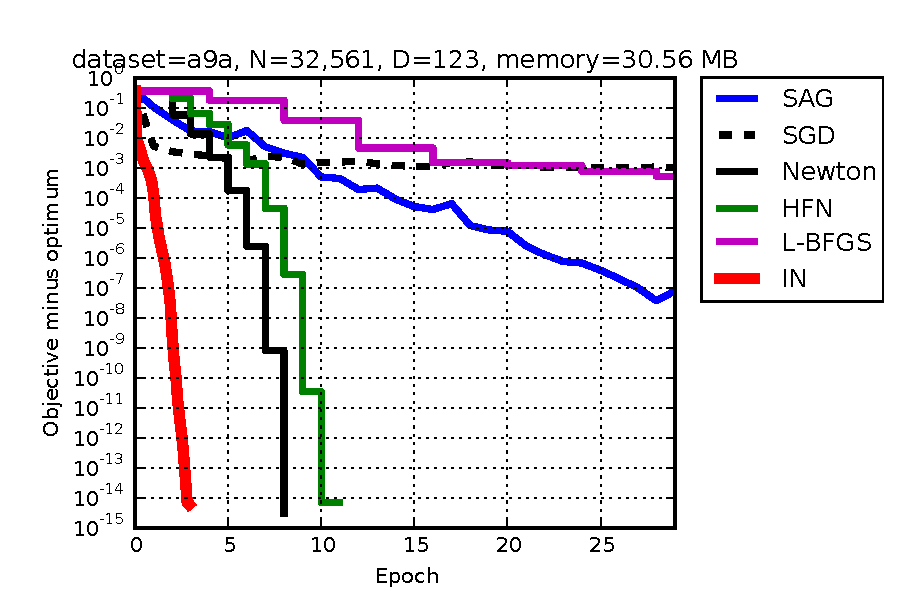
\includegraphics[width=5cm]{a9a_epoch.pdf}
\end{lcode}

Картинка в тексте:
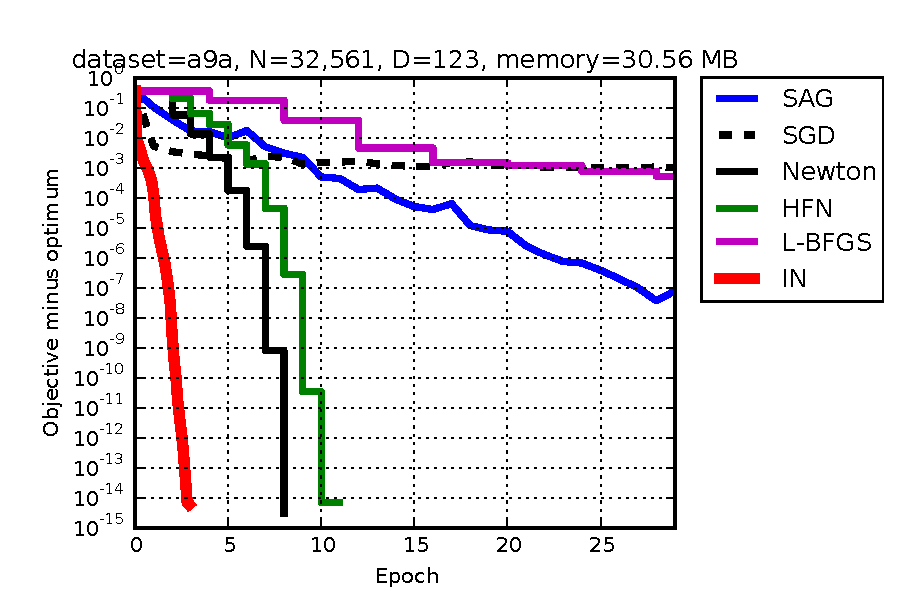
\includegraphics[width=5cm]{a9a_epoch.pdf}
\end{frame}

\begin{frame}[fragile]{Таблица}
\begin{lcode}
    Таблица:
    \begin{tabular}{|cc|c}
        a & b & c \\
        d & e & f \\
    \end{tabular}
\end{lcode}

Таблица:
\begin{tabular}{|cc|c}
    a & b & c \\
    d & e & f \\
\end{tabular}

\end{frame}

\begin{frame}[fragile]{Расположение картинок на странице}

\begin{lcode}
\begin{figure}[h]  %Разместить таблицу здесь
\begin{center}
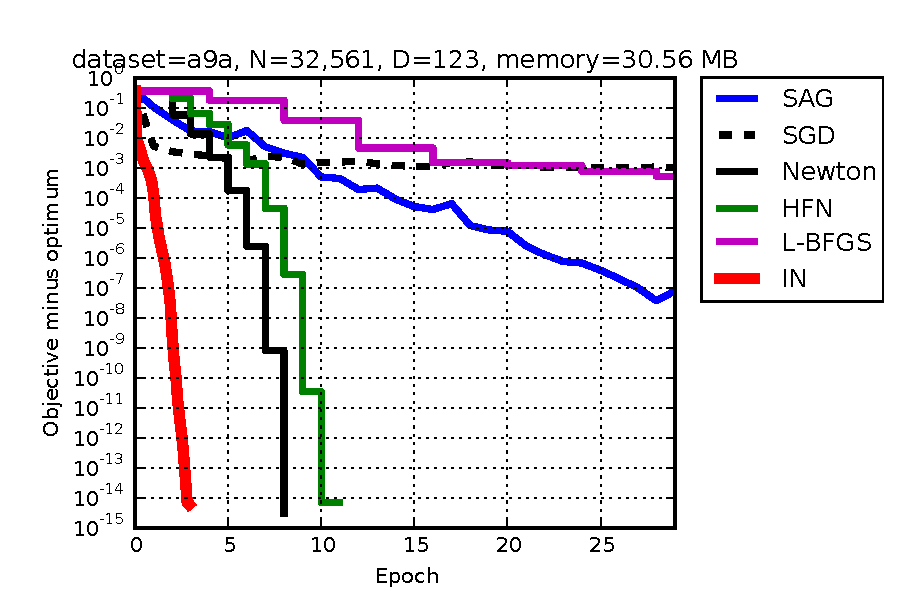
\includegraphics[width=5cm]{a9a_epoch}
\end{center}
\caption{Картинка}\label{fig::1}
\end{figure}

Ссылка на картинку: рис.~\ref{fig::1}
\end{lcode}
\end{frame}

\begin{frame}[fragile]{Несколько картинок на странице}
\small
\begin{lcode}
\tabcolsep = 20pt %длина разделителя между колонками
\begin{tabular}{cc}
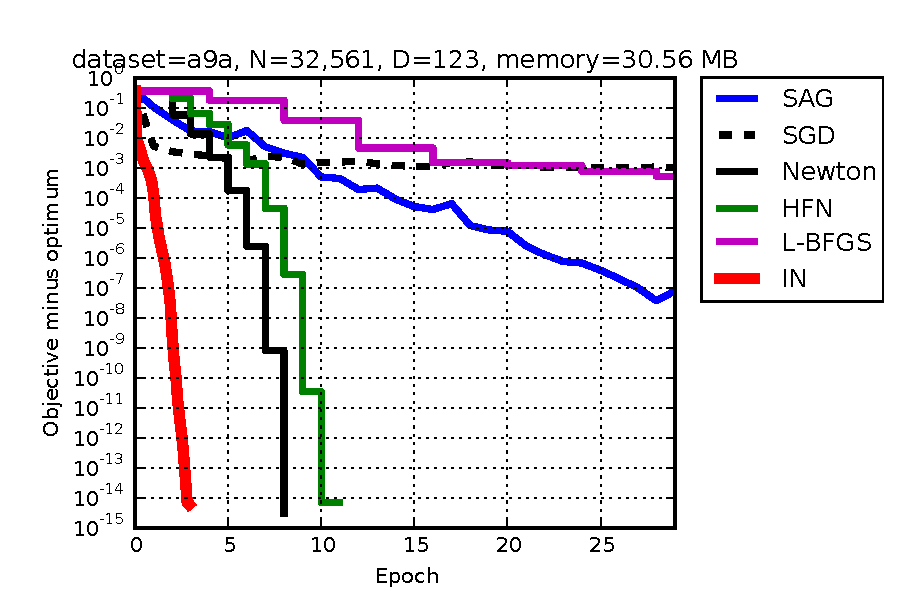
\includegraphics[width=5cm]{a9a_epoch}
&
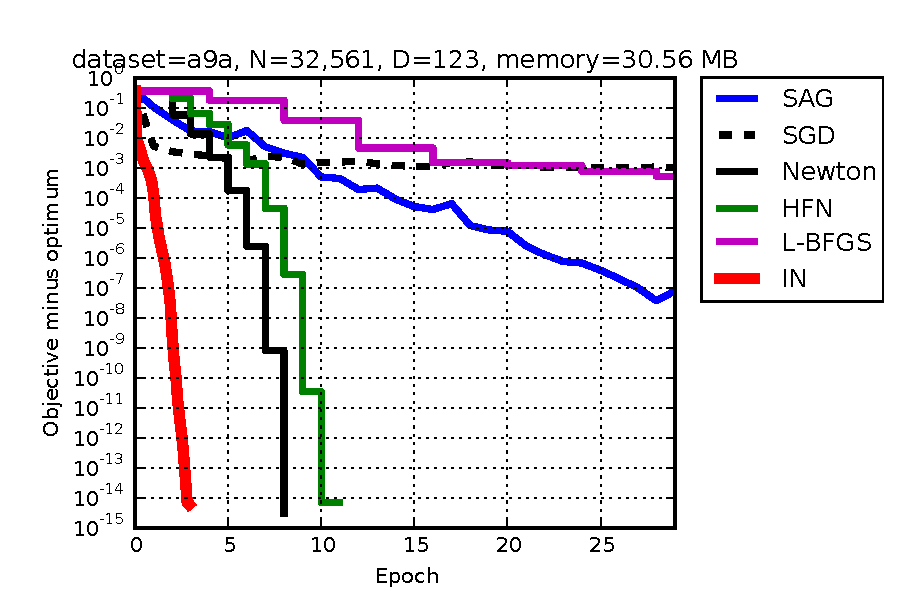
\includegraphics[width=5cm]{a9a_epoch}\\
(a) & (b)
\end{tabular}
\end{lcode}

\begin{center}
    \begin{tabular}{cc}
        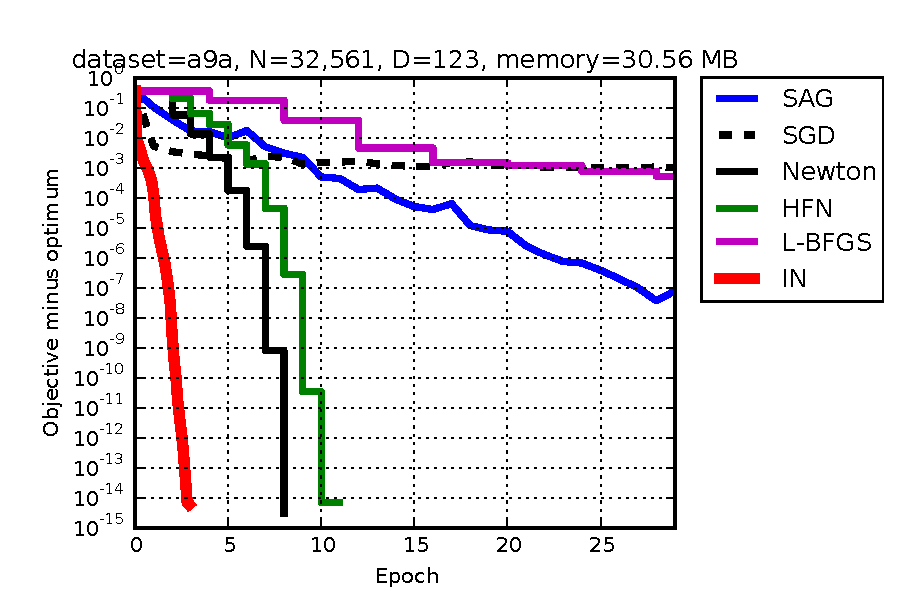
\includegraphics[height=2cm]{a9a_epoch}
        &
        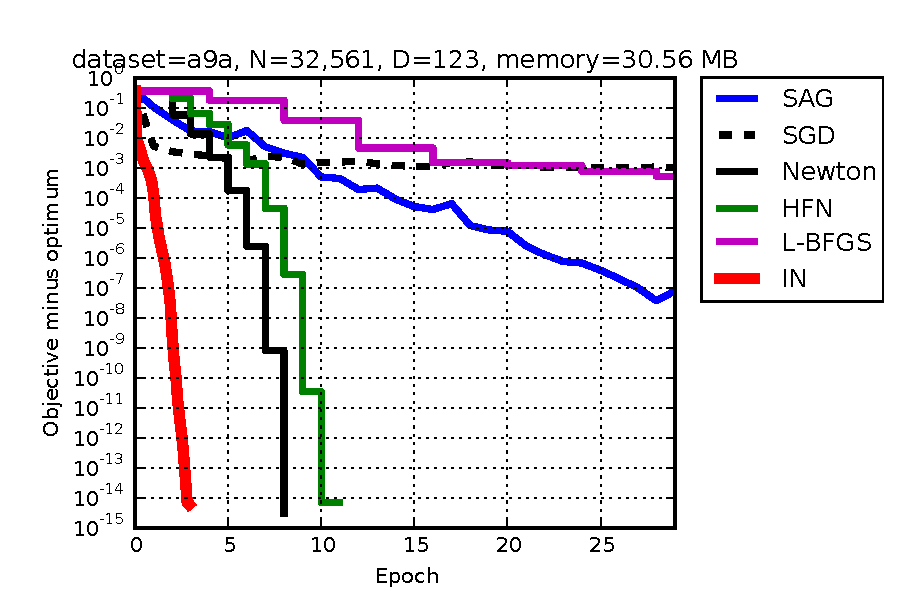
\includegraphics[height=2cm]{a9a_epoch}
        \\
        (a) & (b)
    \end{tabular}
\end{center}
\end{frame}

\begin{frame}[fragile]{Несколько картинок на странице}
    \small
    \begin{lcode}
    \begin{figure}[h]
        \begin{minipage}[b]{0.45\textwidth}\centering
            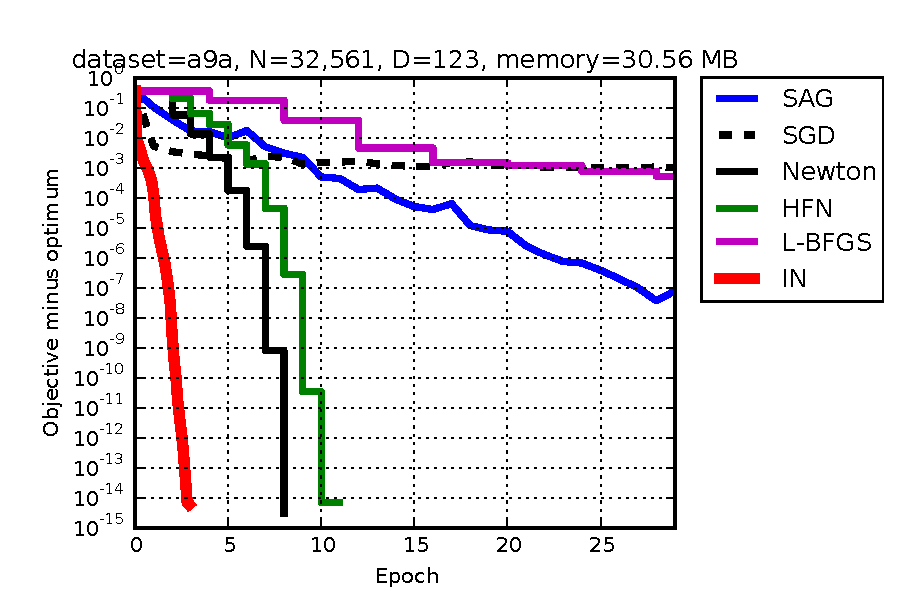
\includegraphics[height=2cm]{a9a_epoch}
        \end{minipage}
        \begin{minipage}[b]{0.45\textwidth}\centering
            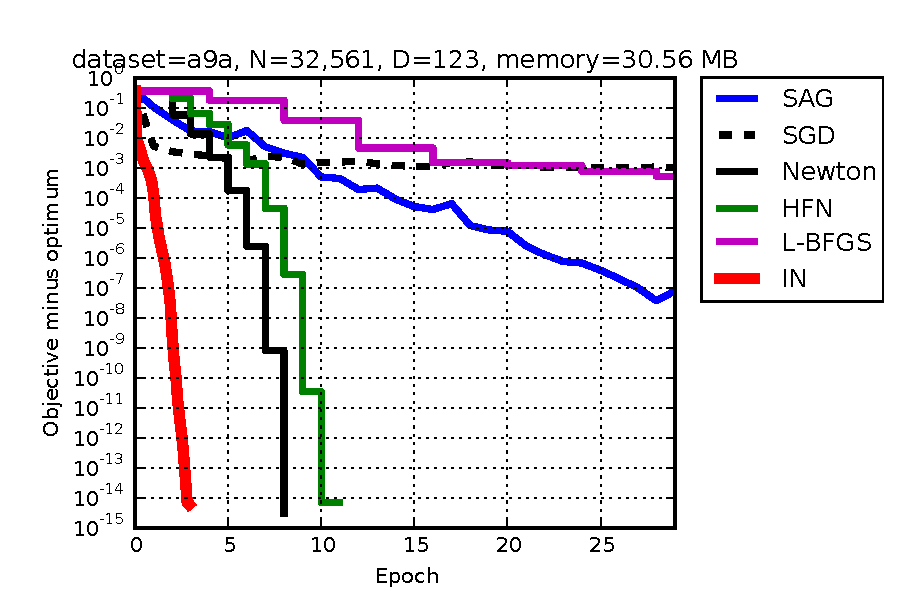
\includegraphics[height=2cm]{a9a_epoch}
        \end{minipage}
    \end{figure}\end{lcode}
    
    \begin{figure}[h]
        \begin{minipage}[b]{0.45\textwidth}\centering
            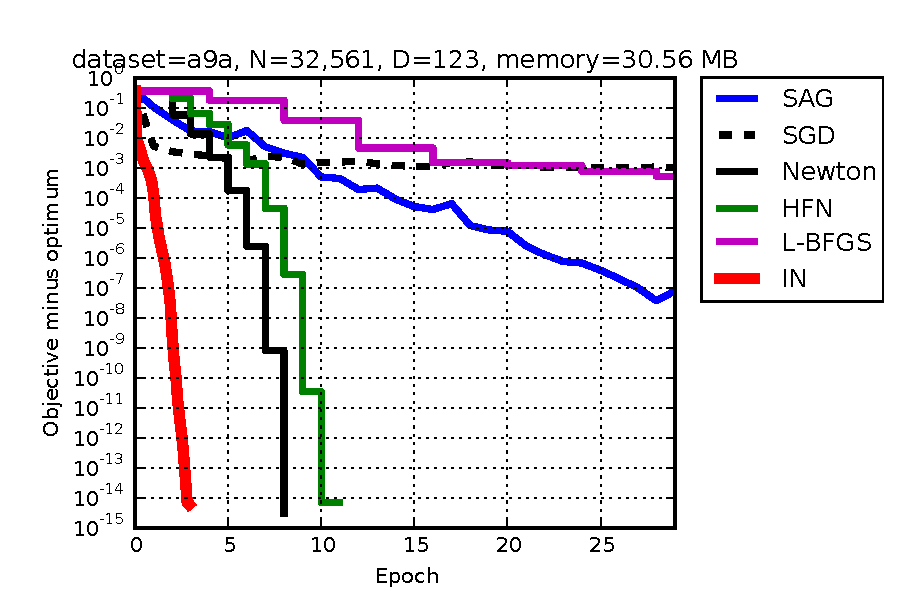
\includegraphics[height=2cm]{a9a_epoch}
        \end{minipage}
        \begin{minipage}[b]{0.45\textwidth}\centering
            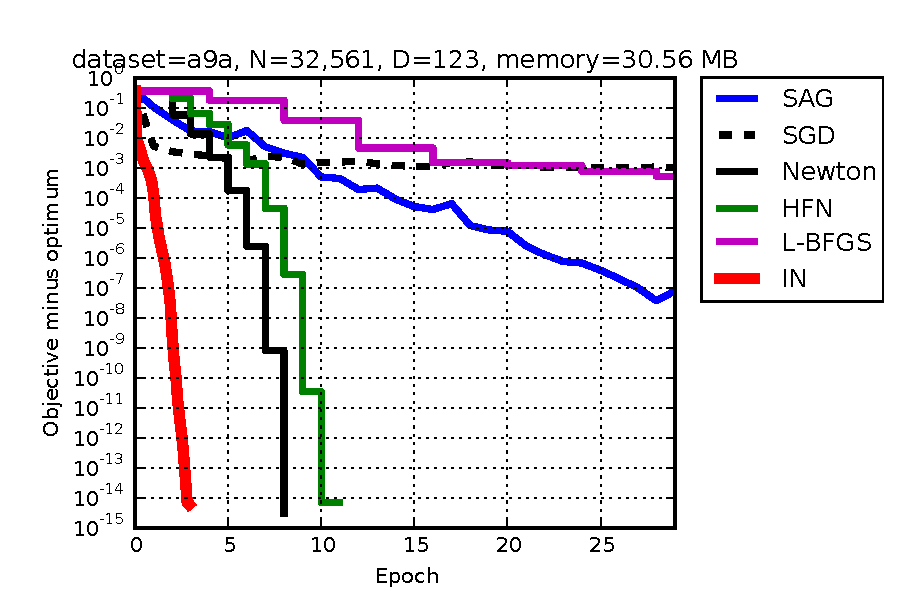
\includegraphics[height=2cm]{a9a_epoch}
        \end{minipage}
    \end{figure}

\end{frame}

\begin{frame}[fragile]{Управление отступами на странице}
    \begin{figure}[h]
        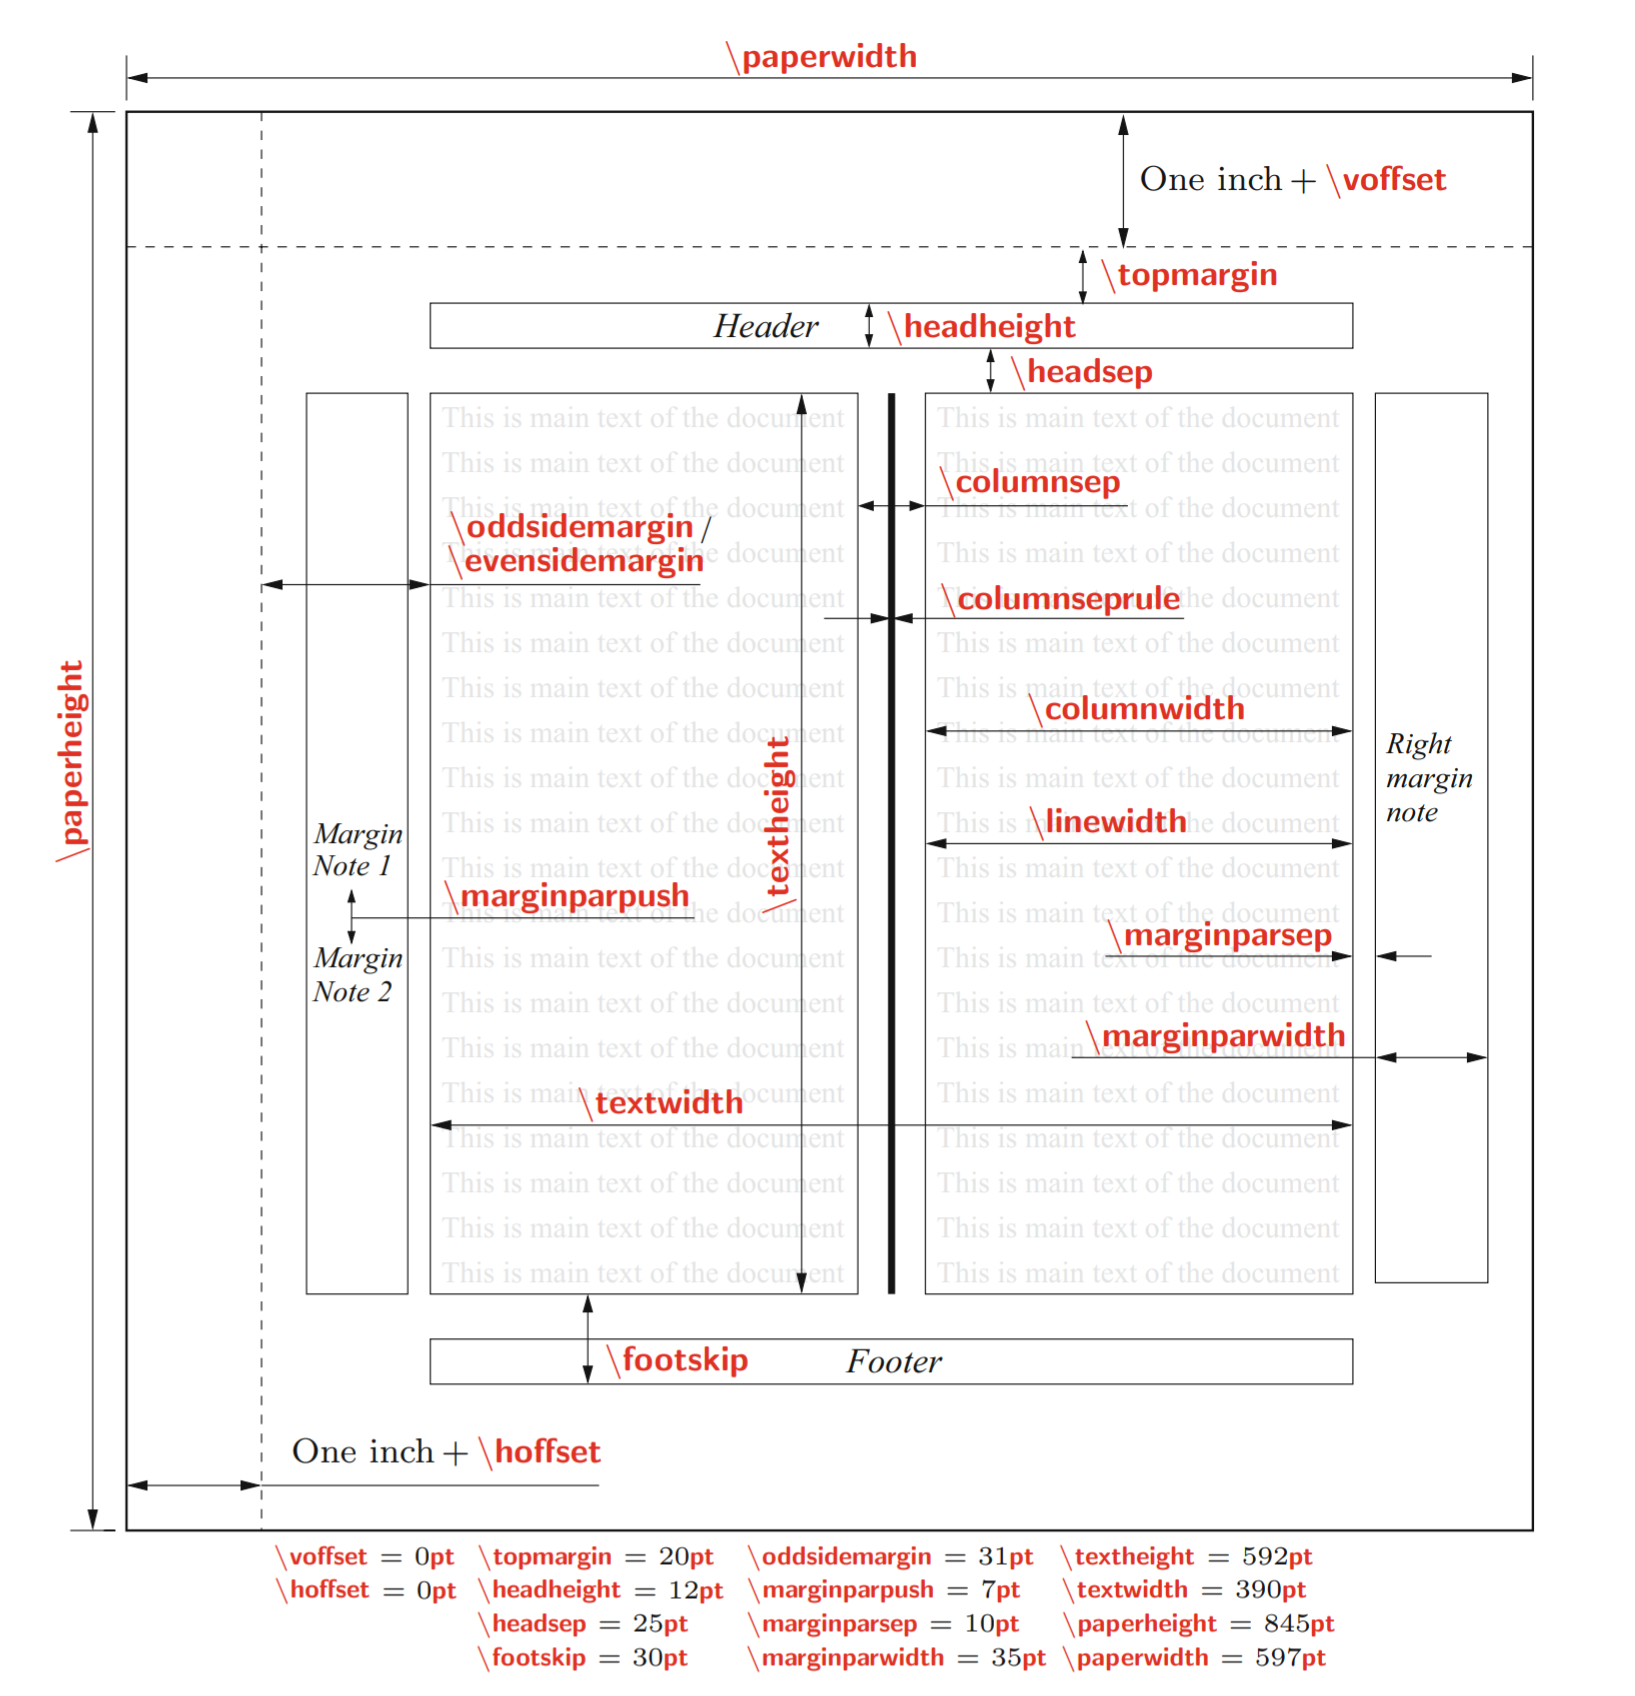
\includegraphics[height=7cm]{Layout.png}
    \end{figure}
\end{frame}

\begin{frame}[fragile]{Несколько команд для управлением текстом}
    \begin{figure}[h]
        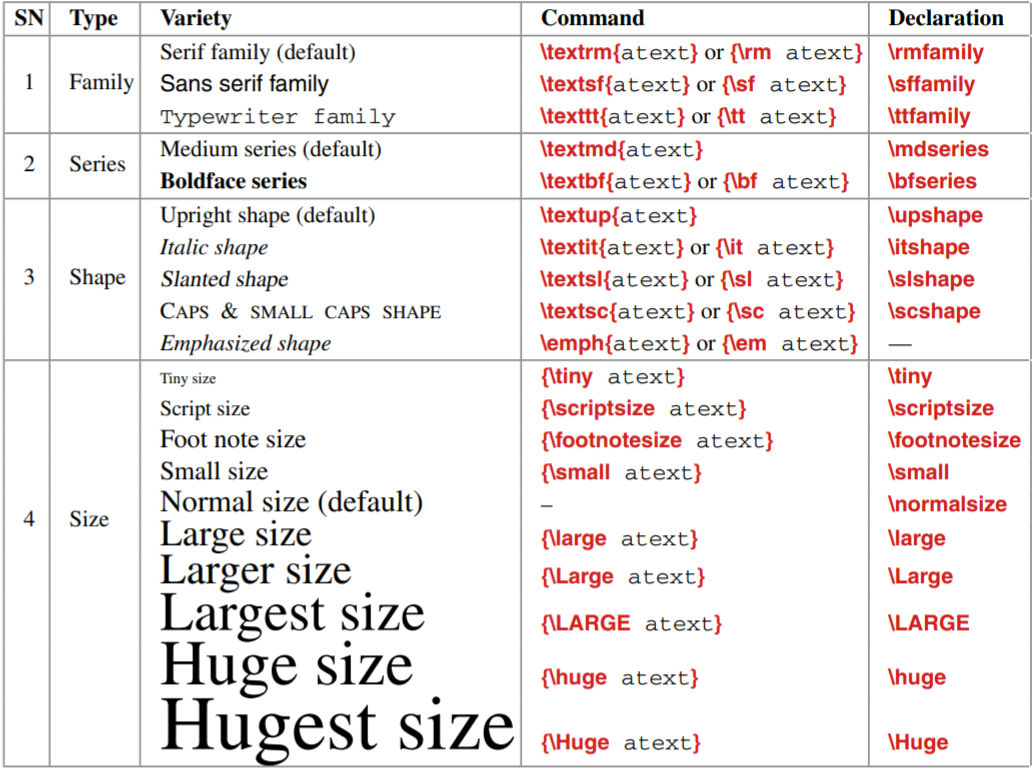
\includegraphics[height=7cm]{Fonts.png}
    \end{figure}
\end{frame}

\begin{frame}[fragile]{Несколько команд для управлением текстом}
    \begin{figure}[h]
        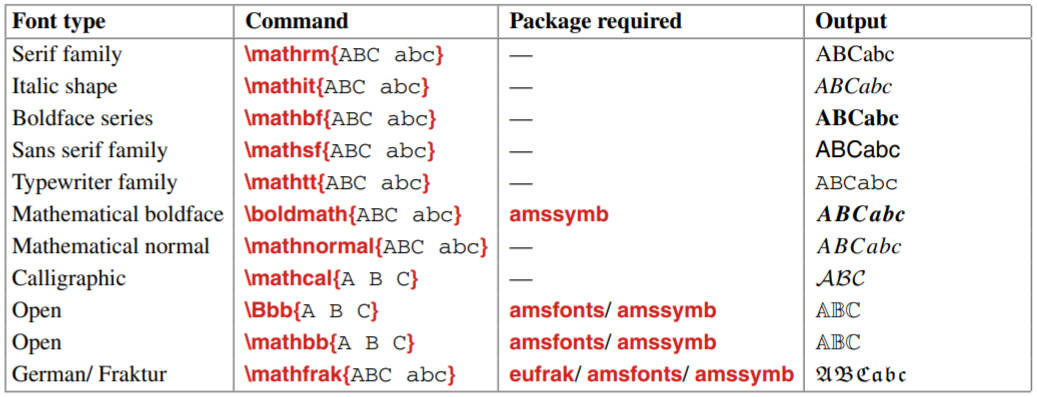
\includegraphics[height=4.5cm]{Math Fonts.png}
    \end{figure}
\end{frame}

\begin{frame}{Особенности типографии: тире и дефис}
\begin{itemize}
    \item дефисы в~словах: из-за $\delta$-функции
          \linline{дефисы в~словах: из-за $\delta$-функции}
          
    \item диапазоны чисел: страницы~3--7
          \linline{диапазоны чисел: страницы~3--7}
          
    \item тире в~предложениях: Это~--- тире.
          \linline{тире в~предложениях: Это~--- тире.}
          
    \item минусы в~формулах: $-f(-x)=f(x)$
          \linline{минусы в~формулах: $-f(-x)=f(x)$}
          
\end{itemize}
\end{frame}

\begin{frame}{Особенности типографии: кавычки}
\begin{itemize}
    \item Французские <<ёлочки>>
    
    \linline{Французские <<ёлочки>>}
    
    \item Немецкие ,,лапки или 99--66‘‘
    
    \linline{Немецкие ,,лапки или 99--66‘‘}
    
    \item Английские ‘‘лапки или 66--99’’
    
    \linline{Английские ‘‘лапки или 66--99’’}
    
    \item Неверно: ,,нигде так не принято’’
    
    \linline{Неверно: ,,нигде так не принято’’}
    
    \item Неверно: ’’и так тоже никто не делает‘‘
    
    \linline{Неверно: ’’и так тоже никто не делает‘‘}
    
    \item Неверно: "а это вообще не кавычки"
    
    \linline{Неверно: "а это вообще не кавычки"}
\end{itemize}
\end{frame}

\begin{frame}[fragile]{Список литературы}
\begin{lcode}
Ссылка в тексте на публикацию~\cite{vorontsovLX}.

% В конце документа
\section{Список литературы}
\begin{thebibliography}{99}
\bibitem{vorontsovUrl}
Воронцов К. В., Полезная информация для
пользователей \LaTeX,
\url{www.ccas.ru/voron/latex.html}

\bibitem{vorontsovLX}
Воронцов К. В., \LaTeX в примерах, 2005,
\url{www.ccas.ru/voron/download/voron05latex.pdf}
\end{thebibliography}
\end{lcode}
\end{frame}

\begin{frame}[fragile]{Список литературы}
\begin{lcode}
Ссылка в тексте на публикацию~\cite{blei06}.
% В конце документа
\section{Список литературы}
\bibliographystyle{gost780s}
\bibliography{references}
\end{lcode}

В файле \texttt{references.bib}:
\begin{lcode}
@ARTICLE{blei06,
author =       {D. Blei and M. Jordan},
title =        {Variational inference for ...},
journal =      {Journal of Bayesian Analysis},
year =         {2006},
volume =       {1},
}
\end{lcode}
\end{frame}

\section{LaTeX и русский язык}
\subsection*{}

\begin{frame}[fragile]\frametitle{BibTeX и русский язык}
BibTex не дружит с кириллицей и utf-8 одновременно!

\hfill

\textbf{Способ 1. } Сохранить файл с библиографией в \texttt{cp1251}, при запуске предупредить о кодировке

(либо вы счастливый обладатель Windows)

\hfill

\begin{lcode}
    \inputencoding{cp1251}
    \bibliographystyle{abbrv}
    \bibliography{liter_cp}
\end{lcode}

\hfill

\end{frame} 

\begin{frame}[fragile]\frametitle{BibTeX и русский язык}
BibTex не дружит с кириллицей и utf-8 одновременно!

\hfill

\textbf{Способ 2. } Использовать при компиляции \texttt{bibtexu} вместо \texttt{bibtex}

(если вы несчастный обладатель Linux)

\hfill

Статья\cite{russianarticle}

\hfill


\begin{lcode}
\bibliography{liter_utf}
\end{lcode}

\hfill


\bibliographystyle{abbrv}
\bibliography{liter_utf}
\end{frame} 

\begin{frame}[fragile]\frametitle{Русский язык в списках}

Переопределить счётчики списков второго уровня на русские буквы:

\begin{lcode}
\renewcommand{\theenumii}{\asbuk{enumii}}
\end{lcode}

\hfill

\renewcommand{\theenumii}{\asbuk{enumii}}

\begin{enumerate}
\item внешний элемент списка;
\item другой внешний элемент;

\begin{enumerate}
\item внутренний элемент 1
\item внутренний элемент 2
\item внутренний элемент 3
\end{enumerate}

\end{enumerate}

\end{frame} 

\section{Подсветка кода}
\subsection*{}


\begin{frame}[fragile]\frametitle{\texttt{verbatim}}
Окружение \linline{verbatim} ---  запрещает LaTeX обрабатывать вставленный текст, отображает код как есть

\begin{verbatim}
def sum(list_of_numbers):
my_sum = 0
for elem in list_of_numbers:
my_sum += elem
return my_sum
\end{verbatim}

\begin{lcode}
    \begin{verbatim}
    def sum(list_of_numbers):
    my_sum = 0
    for elem in list_of_numbers:
    my_sum += elem
    return my_sum
    \end{verbatim}
\end{lcode}

\end{frame} 

\begin{frame}[fragile]\frametitle{Пакет \texttt{listings}}
Пакет \linline{listings} ---  мощный пакет LaTeX, позволяющий настраивать специфическое оформление для кода

\begin{lstlisting}
def sum(list_of_numbers):
my_sum = 0
for elem in list_of_numbers:
my_sum += elem
return my_sum
\end{lstlisting}

\begin{lcode}
\begin{lstlisting}
def sum(list_of_numbers):
my_sum = 0
...
\end{lstlisting}
\end{lcode}

\hfill

Правда, по умолчанию он будет работать почти как \linline{verbatim}...
\end{frame} 


\begin{frame}[fragile]\frametitle{Пакет \texttt{listings}}
\begin{minted}[fontsize=\small]{latex}
\usepackage{listings} 
\usepackage{color}

\lstdefinestyle{myLatexStyle}{
basicstyle=\small\ttfamily,
language={python},
numbersep=5mm, numbers=left, numberstyle=\tiny, 
breaklines=true,frame=single,framexleftmargin=8mm,
xleftmargin=8mm, backgroundcolor=\color{green!5},
frameround=fttt,escapeinside=??, rulecolor=\color{red},
morekeywords={reduce},
keywordstyle=\color[rgb]{0,0,1},                   
commentstyle=\color[rgb]{0.133,0.545,0.133},    
stringstyle=\color[rgb]{0.627,0.126,0.941} 
}
\lstset{style=myLatexStyle}
\end{minted}

\end{frame} 

\begin{frame}[fragile]\frametitle{Пакет \texttt{minted}}
Пакет \linline{minted} ---  пакет LaTeX, позволяющий настраивать оформление кода

\hfill

Плюс \linline{minted} --- большое число предустановленных тем

\begin{minted}[fontsize=\small]{python}
def sum(list_of_numbers):
my_sum = 0
for elem in list_of_numbers:
my_sum += elem
return my_sum
\end{minted}

\begin{lcode}
\begin{minted}[fontsize=\small]{python}
def sum(list_of_numbers):
my_sum = 0
...
\end{minted}

\end{lcode}

\end{frame} 

\begin{frame}[fragile]\frametitle{Пакет \texttt{minted}}
Команда \linline{\mintinline{language}{}} для оформления кода внутри связного текста

\hfill

\begin{lcode}
Команда \mintinline{latex}{\mintinline{language}{}}
для оформления кода внутри связного текста
\end{lcode}


\end{frame} 

\begin{frame}[fragile]\frametitle{Плюсы и минусы различных способов}
\begin{itemize}
\item \linline{verbatim} 
\begin{itemize}
\item[+] Быстро, не требует настройки
\item[--] Отсутствие возможностей настройки
\end{itemize}
\item \linline{lstlisting} 
\begin{itemize}
\item[+] Огромное количество возможностей
\item[--] Красивый результат требует тщательной настройки
\item[--] Сложно задавать свои окружения для разных языков
\end{itemize}
\item \linline{minted} 
\begin{itemize}
\item[+] Огромное количество возможностей
\item[+] Больше число предустановленных тем
\item[+] Легко задавать окружения для разных языков
\item[--] Есть проблемы при установке
\end{itemize}
\end{itemize}

\hfill

При использовании всех этих пакетов объявление слайда приходится записывать так:
\begin{minted}[fontsize=\small]{latex}
\begin{frame}[fragile]\frametitle{Плюсы и минусы
различных способов}
\end{minted}
\end{frame} 

\section{TikZ и PFG}
\subsection*{}
\begin{frame}[fragile]\frametitle{\texttt{TikZ} и \texttt{PFG}}
\texttt{PFG} --- низкоуровневый пакет для векторной графики в \TeX

\hfill

\texttt{TikZ} --- высокоуровневое расширение этого пакета

\hfill

\href{http://www.texample.net/tikz/}{http://www.texample.net/tikz/} --- сайт с примерами работы

\hfill

\href{http://www.texample.net/tikz/}{http://www.texample.net/tikz/} --- сайт с примерами работы

\hfill

\href{http://www.texample.net/media/pgf/builds/pgfmanualCVS2012-11-04.pdf}{короткая ссылка} --- самое подробное~руководство

\end{frame}

\begin{frame}[fragile]\frametitle{Изображение графиков}
\begin{minipage}{0.49\linewidth}
\begin{tikzpicture}[scale=0.6]
\begin{axis}[
%title = Функции пороговой обработки,
line width = 1pt,
xlabel = {$x$},
xtick={-1, 0, 1},
xticklabels={-T, 0, T},
ytick={-1, 0, 1},
yticklabels={-T, 0, T},
mark=none,
legend entries={hard, soft, hybrid},
legend style={legend pos=south east, font=\Large}
]
\addplot[blue] coordinates {(-2, -2) (-1, -1) (-1, 0) (1, 0) (1, 1) (2, 2)};
\addplot[red] coordinates {(-2, -1) (-1, 0) (1, 0) (2, 1)};
\addplot[green, domain=-2:-1] {x - 1/x};
\addplot[green, domain=1:2] {x - 1/x};
\addplot[green, domain=-1:1] {0};
\addplot[blue, dashed] coordinates {(-2, -2) (2, 2)};
\end{axis}
\end{tikzpicture}
\end{minipage}
\begin{minipage}{0.49\linewidth}
\begin{minted}[fontsize=\small]{latex}
\begin{tikzpicture }[scale=0.7]
\begin{axis}[
line width = 1pt,
xlabel = {$x$},
xtick={-1, 0, 1},
xticklabels={-T, 0, T},
ytick={-1, 0, 1},
yticklabels={-T, 0, T},
mark=none,
legend entries={hard, soft,
hybrid},
legend style={font=\Large,
legend pos=south east}
]
...
\end{minted}
\end{minipage}
\end{frame}

\begin{frame}[fragile]\frametitle{Изображение графиков}
\begin{minipage}{0.49\linewidth}
\begin{tikzpicture}[scale=0.6]
\begin{axis}[
%title = Функции пороговой обработки,
line width = 1pt,
xlabel = {$x$},
xtick={-1, 0, 1},
xticklabels={-T, 0, T},
ytick={-1, 0, 1},
yticklabels={-T, 0, T},
mark=none,
legend entries={hard, soft, hybrid},
legend style={legend pos=south east, font=\Large}
]
\addplot[blue] coordinates {(-2, -2) (-1, -1) (-1, 0) (1, 0) (1, 1) (2, 2)};
\addplot[red] coordinates {(-2, -1) (-1, 0) (1, 0) (2, 1)};
\addplot[green, domain=-2:-1] {x - 1/x};
\addplot[green, domain=1:2] {x - 1/x};
\addplot[green, domain=-1:1] {0};
\addplot[blue, dashed] coordinates {(-2, -2) (2, 2)};
\end{axis}
\end{tikzpicture}
\end{minipage}
\begin{minipage}{0.49\linewidth}
\begin{minted}[fontsize=\small]{latex}
...
\addplot[blue] coordinates
{(-2, -2) (-1, -1) (-1, 0)
(1, 0) (1, 1) (2, 2)};
\addplot[blue, dashed] coordinates
{(-2, -2) (2, 2)};
\addplot[red] coordinates ...
\addplot[green, domain=-2:-1]
{x - 1/x};
\addplot[green, domain=1:2]
{x - 1/x};
\addplot[green, domain=-1:1]
{0};
\end{axis}
\end{tikzpicture}

\end{minted}
\end{minipage}

\end{frame}

\begin{frame}[fragile]\frametitle{Изображение линий уровня}
\bigskip
Линии уровня для $\Vert X\vec w-\vec y\Vert_2$ и области $\|w\|_1 \leqslant \kappa, \|w\|_2 \leqslant \kappa$:

\begin{minipage}{0.49\linewidth}
\[
\begin{tikzpicture}
\draw[->] (-1.5, 0) -- (3, 0) node[anchor=north] {$x_1$};
\draw[->] (0, -1.5) -- (0, 3.5) node[anchor=east] {$x_2$};
\draw (-0.2, -0.2) node[scale=0.8] {$0$};
\draw (2, 3.5 ) node {$l_1$-регуляризация};

\draw[blue] (0.83, 2) circle (1.2cm);
\draw[blue] (0.83, 2) circle (0.9cm);
\draw[blue] (0.83, 2) circle (0.6cm);
\draw[blue] (0.83, 2) circle (0.3cm);

\draw[red] (0, -1.1) -- (1.1, 0) -- (0, 1.1) -- (-1.1, 0) -- (0, -1.1);
\filldraw[pattern color=red, pattern=north west lines] (0, -1.1) -- (1.1, 0) -- (0, 1.1) -- (-1.1, 0) -- (0, -1.1);
%\draw[red] (0, -0.83) -- (0.83, 0) -- (0, 0.83) -- (-0.83, 0) -- (0, -0.83);
%\draw[red] (0, -0.5) -- (0.5, 0) -- (0, 0.5) -- (-0.5, 0) -- (0, -0.5);

\node at (0, 1.1) [scale=0.4,shape=circle,draw=blue,fill=blue] {};
\draw (-0.1, 2) -- (0.1, 2);
\draw (-0.2, 1.9) node[scale=0.8] {$y_2$};
\draw (0.83, -0.1) -- (0.83, 0.1);
\draw (0.83 + 0.1, -0.2) node[scale=0.8] {$y_1$};

\end{tikzpicture}
\] 
\end{minipage}
\begin{minipage}{0.49\linewidth}
\[
\begin{tikzpicture}

\draw[->] (-1.5 + 8, 0) -- (3 + 8, 0) node[anchor=north] {$x_1$};
\draw[->] (0 + 8, -1.5) -- (0 + 8, 3.5) node[anchor=east] {$x_2$};
\draw (-0.2 + 8, -0.2) node[scale=0.8] {$0$};
\draw (3.5 + 6.5, 3.5 + 0.2) node {$l_2$-регуляризация};

\draw[blue] (0.83 + 8, 2) circle (1.2cm);
\draw[blue] (0.83 + 8, 2) circle (0.9cm);
\draw[blue] (0.83 + 8, 2) circle (0.6cm);
\draw[blue] (0.83 + 8, 2) circle (0.3cm);

\draw[red] (0.0 + 8, 0) circle (0.94cm);
\filldraw[pattern color=red, pattern=north west lines] (0.0 + 8, 0) circle (0.94cm);
%\draw[red] (0.0 + 8, 0) circle (0.65cm);
%\draw[red] (0.0 + 8, 0) circle (0.4cm);

\node at (0.3 + 8, 0.9) [scale=0.4,shape=circle,draw=blue,fill=blue] {};
\draw (-0.1 + 8, 2) -- (0.1 + 8, 2); % засечка на оси
\draw (-0.2 + 8, 1.9) node[scale=0.8] {$y_2$};
\draw (0.83 + 8, -0.1) -- (0.83 + 8, 0.1);
\draw (0.83 + 0.1 + 8, -0.2) node[scale=0.8] {$y_1$};        
\end{tikzpicture}
\] 
\end{minipage}
\end{frame}
\begin{frame}[fragile]\frametitle{Изображение линий уровня}
\begin{minted}[fontsize=\small]{latex}
\begin{tikzpicture }
\draw[->] (-1.5, 0) -- (3, 0) node[anchor=north] {$x_1$};
\draw[->] (0, -1.5) -- (0, 3.5) node[anchor=east] {$x_2$};
\draw (-0.2, -0.2) node[scale=0.8] {$0$};
\draw (2, 3.5 ) node {$l_1$-регуляризация};

\draw[blue] (0.83, 2) circle (1.2cm);
\draw[blue] (0.83, 2) circle (0.9cm);
\draw[blue] (0.83, 2) circle (0.6cm);
\draw[blue] (0.83, 2) circle (0.3cm);

\draw[red] (0, -1.1) -- (1.1, 0) -- (0, 1.1) --
(-1.1, 0) -- (0, -1.1);
\filldraw[pattern color=red, pattern=north west lines]
(0, -1.1) -- (1.1, 0) -- (0, 1.1) --
(-1.1, 0) -- (0, -1.1);
...
\end{minted}
\end{frame}



\begin{frame}[fragile]\frametitle{Изображение графа}

\begin{minipage}{0.49\linewidth}
\begin{tikzpicture}[scale=2]
\node (p1) at (0,0) [scale=0.6,shape=circle,draw=black,fill=white] {1};
\node (p2) at (2,0) [scale=0.6,shape=circle,draw=black,fill=yellow] {2};
\node (p3) at (1,1) [scale=0.6,shape=circle,draw=red,fill=white] {3};
\node (p4) at (2,2) [scale=0.6,shape=rectangle,draw=black,fill=white] {4};
\node (p5) at (0,2) [scale=0.6,shape=circle,draw=black,fill=white] {5};
\node (p6) at (1,2) [scale=0.6,shape=circle,draw=black,fill=white] {6};

\draw (p1) -- (p3) -- (p5);
\draw (p2) -- (p3) -- (p4);
\draw[->] (p6) -- (p3);
\end{tikzpicture}
\end{minipage}
\begin{minipage}{0.49\linewidth}
\begin{minted}[fontsize=\small]{latex}
\begin{tikzpicture }[scale=2]
\node (p1) at (0,0)
[scale=0.6,shape=circle,
draw=black,fill=white] {1};
\node (p2) at (2,0) [scale=0.6,
shape=circle,draw=black,
fill=yellow] {2};
\node (p3) at (1,1) [scale=0.6,
shape=circle,draw=red,
fill=white] {3};
\node (p4) at (2,2) [scale=0.6,
shape=rectangle,draw=black,
fill=white] {4};
\node (p5) at (0,2) [scale=0.6,
shape=circle,draw=black,
fill=white] {5};
...
\end{minted}
\end{minipage}

\end{frame}

\begin{frame}[fragile]\frametitle{Изображение графа}

\begin{minipage}{0.49\linewidth}
\begin{tikzpicture}[scale=2]
\node (p1) at (0,0) [scale=0.6,shape=circle,draw=black,fill=white] {1};
\node (p2) at (2,0) [scale=0.6,shape=circle,draw=black,fill=yellow] {2};
\node (p3) at (1,1) [scale=0.6,shape=circle,draw=red,fill=white] {3};
\node (p4) at (2,2) [scale=0.6,shape=rectangle,draw=black,fill=white] {4};
\node (p5) at (0,2) [scale=0.6,shape=circle,draw=black,fill=white] {5};
\node (p6) at (1,2) [scale=0.6,shape=circle,draw=black,fill=white] {6};

\draw (p1) -- (p3) -- (p5);
\draw (p2) -- (p3) -- (p4);
\draw[->] (p6) -- (p3);
\end{tikzpicture}
\end{minipage}
\begin{minipage}{0.49\linewidth}
\begin{minted}[fontsize=\small]{latex}
...
\node (p6) at (1,2) [scale=0.6,
shape=circle,draw=black,
fill=white] {6};

\draw (p1) -- (p3) -- (p5);
\draw (p2) -- (p3) -- (p4);
\draw[->] (p6) -- (p3);
\end{minted}
\end{minipage}

\end{frame}



\begin{frame}[fragile]\frametitle{Сохранение графиков экспериментов}
Проблема: провели эксперимент, сохранили график, но...
\begin{center}
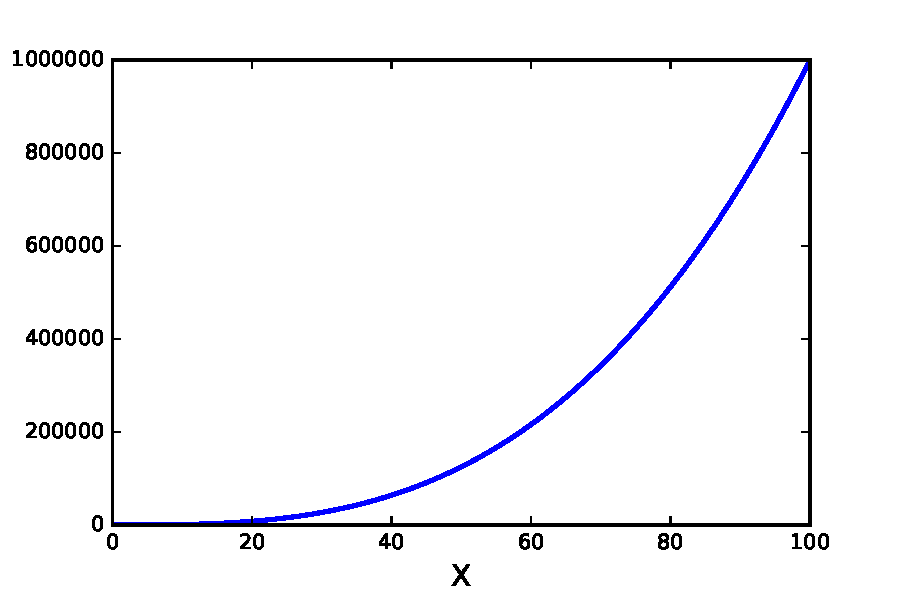
\includegraphics[scale=0.4]{tmp_fig.pdf}
\end{center}

забыли подписать ось $y$.
\end{frame} 

\begin{frame}[fragile]\frametitle{Интеграция \texttt{Python} и \texttt{TikZ}}
Пакет \pinline{matplotlib2tikz} позволяет сохранять графики в формате \linline{TikZ}.

\hfill

\begin{pcode}
import matplotlib.pyplot as plt
from matplotlib2tikz import save as tikz_save

x = [i for i in range(0, 101, 1)]
y = [x_el ** 3 for x_el in x]

plt.plot(x, y, linewidth=2)
plt.xlabel('X', fontsize=14)

tikz_save('tmp_tikz.txt')
\end{pcode}
\end{frame} 

\begin{frame}[fragile]\frametitle{Результат сохранения картинки}
\begin{lcode}
% This file was created by matplotlib2tikz v0.6.13.
\begin{tikzpicture }
\begin{axis}[
xlabel={X},
xmin=0, xmax=100,
ymin=0, ymax=1000000,
axis on top,
tick pos=both
]
\addplot [thick, blue, forget plot]
table {%
0 0
1 1
2 8
...
\end{lcode}
\end{frame}

\begin{frame}[fragile]\frametitle{Вставка картинки в формате \texttt{.tikz}}

\begin{minipage}{0.49\linewidth}
\newlength\figureheight
\newlength\figurewidth
\setlength\figureheight{6cm}
\setlength\figurewidth{6cm}
\input{Figures/tmp_tikz.txt}
\end{minipage}
\begin{minipage}{0.49\linewidth}
\begin{minted}[]{latex}
\newlength\figureheight
\newlength\figurewidth
\setlength\figureheight{6cm}
\setlength\figurewidth{6cm}
\input{tmp_tikz.txt}
\end{minted}
\end{minipage}

\hfill

Что это нам даёт?
\end{frame}

\begin{frame}[fragile]\frametitle{Вставка картинки в формате \texttt{.tikz}}
Картинка сохранена в удобном текстовом представлении

\hfill

Добавим название оси $y$ отредактировав текстовый файл:

\hfill

\begin{minipage}{0.49\linewidth}
\begin{verbatim}
...
\begin{axis}[
xlabel={X},
ylabel={Y},
...
\end{verbatim}
\end{minipage}
\begin{minipage}{0.49\linewidth}
\setlength\figureheight{5cm}
\setlength\figurewidth{5cm}
\input{Figures/tmp_tikz2.txt}
\end{minipage}


\end{frame}

\begin{frame}{Полезные ссылки}
\begin{thebibliography}{}
    
    %Нарисовать текущий элемент в стиле online-ссылки
    \setbeamertemplate{bibliography item}[online]
    \bibitem{lvovsky}
    Львовский~С.\,М. Набор и вёрстка в системе \LaTeX. 2003.
    \url{http://www.ptep-online.com/ctan/llang2003.pdf}
    
    \setbeamertemplate{bibliography item}[online]
    \bibitem{vorontsovLatex}
    Воронцов К. В. \LaTeX\ в примерах, 2005,
    \url{http://www.ccas.ru/voron/download/voron05latex.pdf}
    
    \bibitem{voronstovhints}
    Написание отчётов и статей (рекомендации),
    \href{www.machinelearning.ru/wiki/index.php?title=Категория:Рекомендации_для_студентов}{ссылка}.
    
    \bibitem{baldin}
    Балдин Е.М. LATEX, GNU/Linux и русский стиль,
    \href{http://www.apmath.spbu.ru/cnsa/tex/BaldinEM_LaTEX_v_Rossii.pdf}{ссылка}.
    
    \bibitem{latex_24}
    Dilip Datta. LaTeX in 24 Hours,
    \href{http://www.tezu.ernet.in/dmech/people/ddatta_files/attachment/LaTeX_24H_Note.pdf}{ссылка}.

    \bibitem{cheatlist}
    Шпаргалка по частоиспользуемым математическим символам в \LaTeX,
    \href{https://www.caam.rice.edu/~heinken/latex/symbols.pdf}{ссылка}.
\end{thebibliography}
\end{frame}
\end{document}